\BourbakiExerciseGroup

\begin{enumerate}
\def\labelenumi{\arabic{enumi})}
\tightlist
\item
  Let \(u(\mathbf{X}) = \sum_{n=0}^{\infty} \alpha_n \mathbf{X}^n\) be a formal power series over a commutative field \(\mathbf{K}\) .
\end{enumerate}

\begin{enumerate}
\def\labelenumi{\alph{enumi})}
\tightlist
\item
  For u to be a rational fraction of \(\mathbf{K}(\mathbf{X})\) it is necessary and sufficient that there should exist a finite sequence of elements \((\lambda_{i})_{1\leq i\leq q}\) of elements of K, not all zero, and an integer \(d\geq0\) such that for all \(n\geq d\) we have
\end{enumerate}

\[
\lambda_ {1} \alpha_ {n} + \lambda_ {2} \alpha_ {n + 1} + \dots + \lambda_ {q} \alpha_ {n + q - 1} = 0.
\]

\begin{enumerate}
\def\labelenumi{\alph{enumi})}
\setcounter{enumi}{1}
\tightlist
\item
  Put
\end{enumerate}

\[
\mathrm{H} _ {n} ^ {(k)} = \left| \begin{array}{c c c c} \alpha_ {n} & \alpha_ {n + 1} & \dots & \alpha_ {n + k - 1} \\ \alpha_ {n + 1} & \alpha_ {n + 2} & \dots & \alpha_ {n + k} \\ \alpha_ {n + 2} & \alpha_ {n + 3} & \dots & \alpha_ {n + k + 1} \\ \vdots & \vdots & \ddots & \vdots \\ \alpha_ {n + k - 1} & \alpha_ {n + k} & \dots & \alpha_ {n + 2 k - 2} \end{array} \right|
\]

(« Hankel determinant ») show that if \(\mathrm{H}_{d+j}^{(q+1)} = 0\) and \(\mathrm{H}_{d+j}^{(q)} \neq 0\) for every integer \(j \geqslant 0\) , then \(u(\mathbf{X})\) is a rational fraction (use \(a\) )).

\begin{enumerate}
\def\labelenumi{\alph{enumi})}
\setcounter{enumi}{2}
\tightlist
\item
  Prove the identity
\end{enumerate}

\[
\mathrm{H} _ {n} ^ {(k)} \mathrm{H} _ {n + 2} ^ {(k)} - \mathrm{H} _ {n} ^ {(k + 1)} \mathrm{H} _ {n + 2} ^ {(k - 1)} = (\mathrm{H} _ {n + 1} ^ {(k)}) ^ {2}
\]

(cf.~III, p.~639, Exercise 10). Deduce that if \(\mathrm{H}_{m+j}^{(k+1)} = 0\) for \(0 \leqslant j \leqslant r-1\) , then the \(r\) determinants \(\mathrm{H}_{m+j}^{(k)}\) where \(1 \leqslant j \leqslant r\) are either all zero or all non-zero.

\(d\) ) Deduce from \(b\) ) and \(c\) ) that for \(u(\mathbf{X})\) to be a rational fraction it is necessary and sufficient that there exist two integers \(d\) and \(q\) such that \(\mathrm{H}_{d + j}^{(q + 1)} = 0\) for all integers \(j\geqslant 0\)

\begin{enumerate}
\def\labelenumi{\alph{enumi})}
\setcounter{enumi}{4}
\tightlist
\item
  Let \(k\) be a subfield of \(\mathbf{K}\) , and identify \(\mathbf{K}(\mathbf{X})\) , \(k(\mathbf{X})\) and \(k[[\mathbf{X}]]\) with subrings of \(\mathbf{K}((\mathbf{X}))\) . Prove that \(k[[\mathbf{X}]] \cap \mathbf{K}(\mathbf{X}) = k[[\mathbf{X}]] \cap k(\mathbf{X})\) .
\end{enumerate}

\begin{enumerate}
\def\labelenumi{\arabic{enumi})}
\setcounter{enumi}{1}
\tightlist
\item
  Let \(a_1, a_2, \ldots, a_p\) be integers \(> 0\) ; denote by \(\alpha_n\) the number of finite sequences \((x_i)_{1 \leqslant i \leqslant p}\) of integers \(\geqslant 0\) satisfying the equation
\end{enumerate}

\[
a _ {1} x _ {1} + a _ {2} x _ {2} + \dots + a _ {p} x _ {p} = n.
\]

Show that the formal power series \(\sum_{n=0}^{\infty} \alpha_n X^n\) (over \(\mathbf{Q}\) ) is the expansion of the rational fraction

\[
\frac {1}{(1 - \mathrm{X} ^ {a _ {1}}) (1 - \mathrm{X} ^ {a _ {2}}) \dots (1 - \mathrm{X} ^ {a _ {p}})}.
\]

\begin{enumerate}
\def\labelenumi{\arabic{enumi})}
\setcounter{enumi}{2}
\tightlist
\item
  Let \(\mathbf{F}\) be a finite set of integers \(> 0\) , and let \(\beta_{n}\) be the number of finite sequences \((x_{i})\) of at most \(n\) terms, all of whose terms lie in \(\mathbf{F}\) and such that \(\sum_{i} x_{i} = n\) . Show that the formal power series \(\sum_{n=0}^{\infty} \beta_n X^n\) over \(Q\) is the expansion of the rational fraction
\end{enumerate}

\[
\frac {1}{1 - \sum_ {a \in F} X ^ {a}}.
\]

\begin{enumerate}
\def\labelenumi{\arabic{enumi})}
\setcounter{enumi}{3}
\item
  Let E be a vector space with an infinite basis over a field K of characteristic 2; let B be the exterior algebra \(\Lambda E\) on this space, which is a commutative ring. Give an example of a formal power series \(u \in B[[X]]\) such that \(u^2 = 0\) but such that there exists no element \(\gamma \neq 0\) of B for which \(\gamma u = 0\) .
\item
  Let \(\mathbf{E} = \mathbf{A}[\mathbf{X}_1, \dots, \mathbf{X}_p]\) , \(\mathbf{F} = \mathbf{A}[[\mathbf{X}_1, \dots, \mathbf{X}_p]]\) .
\end{enumerate}

\begin{enumerate}
\def\labelenumi{\alph{enumi})}
\item
  If D is a Z-derivation of E into F, we have \(\omega(Du) \geqslant \omega(u) - 1\) for every non-zero \(u\) in E. b) If D' is a Z-derivation of F, then \(\omega(D'v) \geqslant \omega(v') - 1\) for every non-zero \(v\) in F.
\item
  If E is equipped with the topology induced by that of F, then D and D' are continuous. d) Every Z-derivation of E into F extends in a unique fashion to a Z-derivation of F. e) Let D be the F-module of A-derivations of F. If D ∈ D and DX\_i = u\_i, then D = ∑\_\{i=1\}\^{}\{p\} u\_i D\_i.
\end{enumerate}

\(f)\) \((\mathbf{D}_1,\dots ,\mathbf{D}_p)\) is a basis of the F-module \(\mathcal{D}\) .

\begin{enumerate}
\def\labelenumi{\arabic{enumi})}
\setcounter{enumi}{5}
\tightlist
\item
  Let \((u_{\lambda})_{\lambda \in L}\) be a family of elements of \(\mathbf{A}[[\mathbf{X}_i]]_{i\in I}\) . If the family \((1 + u_{\lambda})_{\lambda \in L}\) is multipliable, the family \((u_{\lambda})_{\lambda \in L}\) is summable.
\end{enumerate}

* 7) If A is reduced, then so is \(\mathbf{A}[[(\mathbf{X}_i)_{i\in I}]]\) . *

\begin{enumerate}
\def\labelenumi{\arabic{enumi})}
\setcounter{enumi}{7}
\tightlist
\item
  We denote by \((1 + \mathbf{X})^{\mathrm{T}}\) the element \(\exp (\mathrm{T}\log (1 + \mathbf{X}))\) of \(\mathbf{Q}[[\mathbf{X},\mathrm{T}]]\) .
\end{enumerate}

\begin{enumerate}
\def\labelenumi{\alph{enumi})}
\tightlist
\item
  Show that \((1 + \mathbf{X})^{\mathrm{T}} = \sum_{n\geqslant 0}\frac{\mathrm{T}(\mathrm{T} - 1)\dots(\mathrm{T} - n + 1)}{n!}\mathbf{X}^{n}\) . (The coefficient of \(\mathbf{X}^n\) is a
\end{enumerate}

polynomial in T whose value is known for \(\mathbf{T} = n\in \mathbf{N}\) .)

\begin{enumerate}
\def\labelenumi{\alph{enumi})}
\setcounter{enumi}{1}
\tightlist
\item
  Show that \((1 + \mathbf{X})^{\mathrm{T}}(1 + \mathbf{X})^{\mathrm{T}} = (1 + \mathbf{X})^{\mathrm{T} + \mathrm{T}}\) . Write down explicitly the identity between binomial coefficients so obtained. Show that \((1 + \mathbf{X} + \mathbf{Y} + \mathbf{XY})^{\mathrm{T}} = (1 + \mathbf{X})^{\mathrm{T}}(1 + \mathbf{Y})^{\mathrm{T}}\) .
\end{enumerate}

\BourbakiExerciseGroup

\begin{enumerate}
\def\labelenumi{\arabic{enumi})}
\tightlist
\item
  (Algebra of sequences of exponential type) Given two integers \(p, q \in \mathbf{N}\) , we denote by \(((p, q))\) the binomial coefficient \(\frac{(p + q)!}{p!q!}\) . Let \(k\) be a commutative ring and \(B\) an associative commutative unital \(k\) -algebra. By a sequence of exponential type of elements of \(B\) we understand a sequence \(a = (a_p)_{p \in \mathbf{N}}\) such that \(a_0 = 1_B\) and \(a_p a_q = ((p, q)) a_{p + q}\) for any \(p, q \in \mathbf{N}\) . The set of all sequences of exponential type of \(B\) is written \(\mathcal{E}(B)\) . \(a)\) Verify that there is on \(\mathcal{E}(B)\) a unique \(k\) -algebra structure such that
\end{enumerate}

\[
\begin{array}{c} (a + b) _ {p} = \sum_ {r + s = p} a _ {r} b _ {s}, \\ (a b) _ {p} = p! a _ {p} b _ {p}, \\ (\lambda a) _ {p} = \lambda^ {p} a _ {p}, \end{array}
\]

for any sequence \(a, b \in \mathcal{E}(\mathbf{B})\) and \(p \in \mathbf{N}, \lambda \in k\) . The mapping \(a \mapsto a_1\) is a homomorphism of the algebra \(\mathcal{E}(\mathbf{B})\) into \(\mathbf{B}\) .

\begin{enumerate}
\def\labelenumi{\alph{enumi})}
\setcounter{enumi}{1}
\item
  Suppose that \(k\) contains a subring isomorphic to \(\mathbf{Q}\) . Show that for every \(x \in B\) the sequence \(f(x)\) defined by \(f(x)_p = \frac{1}{p!} x^p\) is of exponential type. Show that \(f\) is an isomorphism of \(B\) onto \(\mathcal{E}(B)\) .
\item
  Let \(\mathbf{B}'\) be an associative commutative unital \(k\) -algebra and let \(h\) be a homomorphism of \(\mathbf{B}\) into \(\mathbf{B}'\) . For each \(a \in \mathcal{E}(\mathbf{B})\) the sequence \(a'\) defined by \(a_p' = h(a_p)\) for any \(p \in \mathbf{N}\) belongs to \(\mathcal{E}(\mathbf{B}')\) . Show that the mapping \(\mathcal{E}(h): a \mapsto a'\) is a homomorphism of \(\mathcal{E}(\mathbf{B})\) into \(\mathcal{E}(\mathbf{B}')\) . Verify that \(\mathcal{E}(g \circ h) = \mathcal{E}(g) \circ \mathcal{E}(h)\) when \(g\) and \(h\) are composable \(k\) -algebra homomorphisms.
\item
  Let E be a \(k\) -module and \(\mathbf{TS}(\mathbf{E})\) the algebra of symmetric tensors on E. Show that for each \(x \in \mathbf{E}\) , \((\gamma_p(x))\) is a sequence of exponential type in the algebra \(\mathbf{TS}(\mathbf{E})\) (IV, p.~45).
\end{enumerate}

\begin{enumerate}
\def\labelenumi{\arabic{enumi})}
\setcounter{enumi}{1}
\tightlist
\item
  (Functor \(\Gamma\) ) Denote by \(k\) a commutative ring and by E a \(k\) -module. By the gamma algebra of E we understand the associative commutative unital algebra defined by the generating system \(\mathbf{N} \times \mathbf{E}\) and by the relators (cf.~III, p.~450)
\end{enumerate}

\[
\begin{array}{c} (0, x) - 1, \\ (p, \lambda x) - \lambda^ {p} (p, x), \\ (p, x + y) - \sum_ {r + s = p} (r, x) (s, y), \\ (p, x) (q, x) - ((p, q)) (p + q, x), \end{array}
\]

where \(p, q\) range over \(\mathbf{N}, x, y\) range over \(\mathbf{E}\) and \(\lambda\) over \(k\) . This algebra is denoted by \(\Gamma(\mathbf{E})\) . For each \(p \in \mathbf{N}\) we denote by \(\gamma_p\) the mapping of \(\mathbf{E}\) into \(\Gamma(\mathbf{E})\) composed of the injection \(x \mapsto (p, x)\) and the canonical homomorphism of the free commutative algebra on \(\mathbf{N} \times \mathbf{E}\) into \(\Gamma(\mathbf{E})\) .

\begin{enumerate}
\def\labelenumi{\alph{enumi})}
\item
  Verify that for each \(x \in \mathbb{E}\) , the sequence \(\gamma_p(x)\) is a sequence of exponential type of elements of \(\Gamma(\mathbb{E})\) (Exercise 1) and that the mapping \(\gamma : x \mapsto (\gamma_p(x))_{p \in \mathbb{N}}\) is a homomorphism of the \(k\) -module \(\mathbb{E}\) into the \(k\) -algebra \(\mathcal{E}(\Gamma(\mathbb{E}))\) .
\item
  (Universal property of \(\Gamma(\mathrm{E})\) ). Let B be an associative commutative unital k-algebra and \(\varphi\) a homomorphism of the k-module E into \(\mathcal{E}(\mathrm{B})\) . Show that there exists a unique algebra homomorphism \(h: \Gamma(\mathrm{E}) \to \mathrm{B}\) such that \(\varphi = \mathcal{E}(h) \circ \gamma\) .
\item
  Show that there exists a unique unital homomorphism of algebras \(\varepsilon : \Gamma(E) \to k\) such that \(\varepsilon(\gamma_p(x)) = 0\) for all \(p > 0\) and all \(x \in E\) .
\end{enumerate}

\(d)\) For each \(p \in \mathbb{N}\) let \(\Gamma_p(E)\) be the submodule of \(\Gamma(E)\) generated by the elements

\[
\gamma_ {\nu_ {1}} (x _ {1}) \dots \gamma_ {\nu_ {s}} (x _ {s})
\]

where \(s \in \mathbf{N}\) , \(\nu \in \mathbf{N}^s\) and \(|\nu| = \sum_{i} \nu_i = p\) . Verify that the submodules \(\Gamma_p(\mathrm{E})\) form a

graduation of the algebra \(\Gamma(E)\) . Show that \(\gamma_{1}\) is an isomorphism of \(E\) onto \(\Gamma_{1}(E)\) (to verify that \(\gamma_{1}\) is injective, consider the algebra \(B = k \times E\) with the product defined by the formula \((\lambda, x)(\mu, y) = (\lambda \mu, \lambda y + \mu x)\) and show that there exists a homomorphism of \(\Gamma(E)\) into \(B\) which maps \(\gamma_{1}(x)\) to \((0, x)\) for any \(x \in E\) ).

\begin{enumerate}
\def\labelenumi{\alph{enumi})}
\setcounter{enumi}{4}
\item
  Let E and F be two k-modules and h a homomorphism of E into F. Show that there exists a unique homomorphism of graded algebras \(\Gamma(h):\Gamma(\mathrm{E})\to\Gamma(\mathrm{F})\) such that \(\gamma_{p}\circ h=\Gamma(h)\circ\gamma_{p}\) for all \(p\in N\) . Verify that if g and h are homomorphisms of k-modules such that \(g\circ h\) is defined, then \(\Gamma(g\circ h)=\Gamma(g)\circ\Gamma(h)\) .
\item
  Let \(h: \mathbf{E} \to \mathbf{F}\) be a surjective homomorphism of \(k\) -modules. Show that \(\Gamma(h)\) is surjective and that its kernel is the ideal of \(\Gamma(\mathbf{E})\) generated by the elements \(\gamma_p(x)\) with \(p > 0\) and \(x \in \operatorname{Ker}(h)\) .
\item
  Let E and F be two k-modules. Show that there exists a unique homomorphism \(\varphi\) of the algebra \(\Gamma(E \times F)\) into the algebra \(\Gamma(E) \otimes_{k} \Gamma(F)\) such that
\end{enumerate}

\[
(\varphi \circ \gamma_ {p}) (x, y) = \sum_ {r + s = p} \gamma_ {r} (x) \otimes \gamma_ {s} (y)
\]

for any \(p \in \mathbf{N}\) , \(x \in E\) and \(y \in F\) . Show that this homomorphism is an isomorphism compatible with the graduations.

\begin{enumerate}
\def\labelenumi{\arabic{enumi})}
\setcounter{enumi}{2}
\tightlist
\item
  Let \(k\) be a commutative ring and \(E\) a \(k\) -module. Show that there exists a unique homomorphism \(\Delta\) of the algebra \(\Gamma(E)\) (Exercise 2) into the algebra \(\Gamma(E) \otimes_k \Gamma(E)\) such that
\end{enumerate}

\[
(\Delta \circ \gamma_ {p}) (x) = \sum_ {r + s = p} \gamma_ {r} (x) \otimes \gamma_ {s} (x)
\]

for all \(x \in E\) and all \(p \in N\) . Show that the coproduct \(\Delta\) is coassociative, cocommutative (III, p.~580-581) and defines on \(\Gamma(E)\) a graded bigebra structure (III, p.~585). Show that the homomorphism \(\varepsilon\) defined in Exercise 2, c) is a counit.

\begin{enumerate}
\def\labelenumi{\arabic{enumi})}
\setcounter{enumi}{3}
\item
  Let \(E_{1}\) and \(E_{2}\) be two modules over a commutative ring k and let h be a homomorphism of \(E_{1}\) into \(E_{2}\) . Verify that \(\Gamma(h)\) (Exercise 2, e)) is a homomorphism of graded bigebras (cf.~Exercise 3).
\item
  Let \(\Gamma(\mathbf{Z})\) be the gamma algebra of the \(\mathbf{Z}\) -module \(\mathbf{Z}\) (Exercise 2). For each \(p \in \mathbf{N}\) put \(\mathrm{T}^{(p)} = \gamma_p(1)\) .
\end{enumerate}

\begin{enumerate}
\def\labelenumi{\alph{enumi})}
\tightlist
\item
  Show that \((\mathbf{T}^{(p)})_{p\in \mathbb{N}}\) is a basis of the \(\mathbf{Z}\) -module \(\Gamma (\mathbf{Z})\) . Show that there exists a unique homomorphism \(\theta\) of the algebra \(\Gamma (\mathbf{Z})\) into the algebra \(\Gamma (\mathbf{Z})\otimes \Gamma (\mathbf{Z})\) such that
\end{enumerate}

\[
\theta \left(\mathrm{T} ^ {(p)}\right) = p! \mathrm{T} ^ {(p)} \otimes \mathrm{T} ^ {(p)}
\]

for all \(p \in \mathbf{N}\) .

\begin{enumerate}
\def\labelenumi{\alph{enumi})}
\setcounter{enumi}{1}
\item
  Let B be a commutative ring and H the set of homomorphisms of the ring \(\Gamma(\mathbf{Z})\) into the ring B. Show that for every \(f \in H\) the sequence \(f(\mathrm{T}^{(p)})\) , \(p \in N\) is a sequence of exponential type of elements of B. Show that the mapping \(\varphi: f \mapsto (f(\mathrm{T}^{(p)}))_{p \in \mathbb{N}}\) is a bijection of H onto \(\mathcal{E}(\mathbf{B})\) (Exercise 1).
\item
  For \(f, g \in \mathbf{H}\) denote by \(f * g\) the homomorphism of \(\Gamma(\mathbf{Z}) \otimes \Gamma(\mathbf{Z})\) into \(\mathbf{B}\) defined by \((f * g)(u \otimes v) = f(u)g(v)\) for any \(u, v \in \Gamma(\mathbf{Z})\) . Verify that for any \(f, g \in \mathbf{H}\) we have
\end{enumerate}

\[
\begin{array}{c} \varphi (f) + \varphi (g) = \varphi ((f * g) \circ \Delta), \\ \varphi (f) \varphi (g) = \varphi ((f * g) \circ \theta). \end{array}
\]

\begin{enumerate}
\def\labelenumi{\arabic{enumi})}
\setcounter{enumi}{5}
\item
  Let \(n\) be an integer \(> 0\) and let \(\Gamma(\mathbf{Z}/n\mathbf{Z})\) be the gamma algebra of the \(\mathbf{Z}\) -module \(\mathbf{Z}/n\mathbf{Z}\) (Exercise 2). Show that for every \(p > 0\) , \(\Gamma_p(\mathbf{Z}/n\mathbf{Z})\) is isomorphic to the quotient of \(\mathbf{Z}\) by the subgroup generated by the integers \(n^k((k, p - k))\) , where \(1 \leqslant k \leqslant p\) . Show that if \(p\) and \(n\) are distinct primes, then \(\Gamma_p(\mathbf{Z}/n\mathbf{Z})\) is cyclic of order \(n\) . Show that if \(n\) is even, then \(\Gamma_2(\mathbf{Z}/n\mathbf{Z})\) is cyclic of order \(2n\) .
\item
  (Extension of scalars) Let \(k\) be a commutative ring, \(L\) an associative commutative unital \(k\) -algebra and \(E\) a \(k\) -module.
\end{enumerate}

\begin{enumerate}
\def\labelenumi{\alph{enumi})}
\tightlist
\item
  Let \(\Gamma(L \otimes_k E)\) be the gamma algebra of the L-module \(L \otimes_k E\) (Exercise 2). Show that there exists a unique homomorphism \(\theta\) of \(L \otimes_k \Gamma(E)\) into \(\Gamma(L \otimes_k E)\) compatible with the algebra structure on \(L\) and such that
\end{enumerate}

\[
\theta (1 \otimes \gamma_ {p} (x)) = \gamma_ {p} (1 \otimes x)
\]

for all \(x \in \mathbf{E}\) and \(p \in \mathbf{N}\) .

\begin{enumerate}
\def\labelenumi{\alph{enumi})}
\setcounter{enumi}{1}
\tightlist
\item
  Show that \(\theta\) is an isomorphism of graded bigebras over \(L\) .
\end{enumerate}

\begin{enumerate}
\def\labelenumi{\arabic{enumi})}
\setcounter{enumi}{7}
\tightlist
\item
  Let \(k\) be a commutative ring and \(E\) a \(k\) -module.
\end{enumerate}

\begin{enumerate}
\def\labelenumi{\alph{enumi})}
\tightlist
\item
  Show that there exists a unique homomorphism g of the algebra \(\Gamma(\mathrm{E})\) (Exercise 2) into the algebra TS(E) of symmetric tensors over E (IV, p.~43) such that
\end{enumerate}

\[
(g \circ \gamma_ {p}) (x) = x \otimes x \otimes \dots \otimes x \quad (p \text {   factors   } x),
\]

for any \(x \in \mathbb{E}\) , \(p \in \mathbb{N}\) . Show that if \(\mathbb{E}\) is a free \(k\) -module with basis \((e_i)_{i \in I}\) , then \(g\) is an isomorphism of graded bigebras (cf.~Exercise 3 and IV, p.~51) and the elements \(\gamma_\alpha = \prod_i \gamma_{\alpha(i)}(e_i)\) , where \(\alpha \in \mathbf{N}^{(I)}\) , form a basis of \(\Gamma(\mathbb{E})\) .

\begin{enumerate}
\def\labelenumi{\alph{enumi})}
\setcounter{enumi}{1}
\tightlist
\item
  Let \(\xi\) be a mapping of \((1, n)\) into \(\mathbf{N}\) and let \(p = \sum_{i=1}^{n} \xi(i)\) . Show that for every sequence
\end{enumerate}

\(x_{1}, x_{2}, \ldots, x_{n}\) of elements of E, the image of \(\gamma_{\xi(1)}(x_{1}) \ldots \gamma_{\xi(n)}(x_{n})\) under \(g\) is \(\sum_{\varphi} x_{\varphi(1)} \otimes \ldots \otimes x_{\varphi(p)}\) where \(\varphi\) runs over the set of all mappings of \([1, p]\) into \([1, n]\) such that

Card \(\varphi^{-1}(i) = \xi(i)\) for each \(i \in [1, n]\) (cf.~IV, p.~45, Prop. 3).

\begin{enumerate}
\def\labelenumi{\alph{enumi})}
\setcounter{enumi}{2}
\tightlist
\item
  Let \(f\) be the mapping of \(\otimes^p \mathbf{E}\) into \(\Gamma_p(\mathbf{E})\) defined by \(f(x_1 \otimes \ldots \otimes x_p) = \gamma_1(x_1) \ldots \gamma_1(x_p)\) for any \(x_1, \ldots, x_p \in \mathbf{E}\) . Show that for each tensor \(t \in \otimes^p \mathbf{E}\) , \((g \circ f)(t)\) is the symmetrization of \(t\) . Show that for each \(u \in \Gamma_p(\mathbf{E})\) we have \((f \circ g)(u) = p! u\) .
\end{enumerate}

\begin{enumerate}
\def\labelenumi{\arabic{enumi})}
\setcounter{enumi}{8}
\tightlist
\item
  (Polynomial laws) Denote by E and F two modules over the commutative ring k. By a polynomial law of E in F we understand, for each (associative commutative and unital) k-algebra L, a mapping \(\varphi_{L}\) of \(L \otimes_{k} E\) into \(L \otimes_{k} F\) satisfying the condition:
\end{enumerate}

If L and R are two k-algebras and f is a unital homomorphism of L into R, then

\[
(f \otimes 1) \circ \varphi_ {L} = \varphi_ {R} \circ (f \otimes 1).
\]

\begin{enumerate}
\def\labelenumi{\alph{enumi})}
\tightlist
\item
  Let \(\varphi\) be a polynomial law of \(E\) into \(F\) , let \(L = k[(T_i)_{i \in I}]\) be the polynomial algebra in a family of indeterminates \(T_i\) over \(k\) and let \((x_i)_{i \in I}\) be a family of finite support of elements of \(E\) . Show that there exists a unique family of finite support \((y_\xi)_{\xi \in N^{(I)}}\) of elements of \(F\) such that
\end{enumerate}

\[
\varphi_ {L} \left(\sum_ {i} T _ {i} \otimes x _ {i}\right) = \sum_ {\xi \in N ^ {(I)}} T ^ {\xi} \otimes y _ {\xi}.
\]

Show that if \(\mathbf{R}\) is an algebra over \(k\) , then for every family \((a_i)_{i \in I}\) of elements of \(\mathbf{R}\) we have

\[
\varphi_ {R} \left(\sum_ {i} a _ {i} \otimes x _ {i}\right) = \sum_ {\xi \in \mathbf {N} ^ {(I)}} a ^ {\xi} \otimes y _ {\xi}.\tag{1}
\]

\begin{enumerate}
\def\labelenumi{\alph{enumi})}
\setcounter{enumi}{1}
\tightlist
\item
  A family \((\varphi^j)_{j \in \mathbb{J}}\) of polynomial laws of E into F is called summable if for every algebra L over \(k\) and every \(u \in \mathrm{L} \otimes \mathrm{E}\) , the family \(\varphi_L^j(u)\) has finite support. Show that if \((\varphi^j)_{j \in \mathbb{J}}\) is a summable family of polynomial laws of E into F, then there exists a unique polynomial law \(\varphi\) of E into F such that for every \(k\) -algebra L and every \(u \in \mathrm{L} \otimes \mathrm{E}\) we have \(\sum_j \varphi_L^j(u) = \varphi_L(u)\) . This polynomial law is called the sum of the laws \(\varphi^j\) and is denoted by
\end{enumerate}

\[
\sum_ {j} \varphi^ {j}.
\]

\begin{enumerate}
\def\labelenumi{\alph{enumi})}
\setcounter{enumi}{2}
\item
  Let E, F, G be three k-modules, \(\varphi\) a polynomial law of E into F and \(\psi\) a polynomial law of F into G. Show that there exists a unique polynomial law \(\eta\) of E into G such that for every k-algebra L we have \(\eta_{L} = \psi_{L} \circ \varphi_{L}\) . This law \(\eta\) is called the composition of \(\varphi\) and \(\psi\) and is denoted by \(\psi \circ \varphi\) .
\item
  Let \(p\) be an integer \(\geqslant 0\) . A polynomial law \(\varphi\) of \(E\) into \(F\) is said to be homogeneous of degree \(p\) if for every algebra \(L\) over \(k\) we have \(\varphi_{L}(au) = a^{p}\varphi_{L}(u)\) for any \(a \in L\) and \(u \in L \otimes E\) . Show that if \(\varphi\) is homogeneous of degree \(p\) , then in formula (1) we have \(y_{\xi} = 0\) for \(|\xi| = \sum_{i} \xi(i) \neq p\) . Determine all homogeneous polynomial laws of degrees 0 and 1.
\item
  With the same notation as in c), show that if \(\varphi\) and \(\psi\) are homogeneous laws of degrees \(p\) and \(q\) respectively, then \(\psi \circ \varphi\) is a homogeneous law of degree \(pq\) .
\item
  Let \(p\) be an integer \(\geqslant 0\) . For every commutative \(k\) -algebra \(L\) we denote by \(\varepsilon_L\) the injection \(a \mapsto aT\) of \(L\) into the polynomial algebra \(L[T]\) and by \(\beta_L^p\) the homomorphism of the \(L\) -module \(L[T]\) into \(L\) which associates with each element \(\sum_k a_k T^k \in L[T]\) the coefficient \(a_p\) . Let \(\varphi\) be a polynomial law of \(E\) into \(F\) . Show that the
\end{enumerate}

mappings \(\varphi_{L}^{p} = (\beta_{L}^{p}\otimes \mathrm{Id}_{F})\circ \varphi_{L[T]}\circ (\varepsilon_{L}\otimes \mathrm{Id}_{E})\) form a polynomial law of E into F which is homogeneous of degree \(p\) . This polynomial law is called the homogeneous component of degree \(p\) of the law \(\varphi\) . Show that the homogeneous components of \(\varphi\) form a summable family with sum \(\varphi\) .

\begin{enumerate}
\def\labelenumi{\arabic{enumi})}
\setcounter{enumi}{9}
\tightlist
\item
  Denote by \(k\) a commutative ring and by \(E\) a \(k\) -module. For each integer \(p \geqslant 0\) and every \(k\) -algebra \(L\) we denote by \(\gamma_{p,L}\) the mapping of \(L \otimes E\) into \(L \otimes \Gamma_p(E)\) composed of \(\gamma_p: L \otimes E \to \Gamma_p(L \otimes E)\) and the canonical isomorphism of \(\Gamma_p(L \otimes E)\) onto \(L \otimes \Gamma_p(E)\) (cf.~Exercises 2 and 7).
\end{enumerate}

\begin{enumerate}
\def\labelenumi{\alph{enumi})}
\tightlist
\item
  Verify that the mappings \(\gamma_{p,L}\) form a polynomial law (Exercise 9) of E into \(\Gamma_p(E)\) , which is homogeneous of degree \(p\) ; this law will in what follows be denoted by \(\boldsymbol{\gamma}_p\) . Show that for every \(k\) -module F and every \(\sigma \in \operatorname{Hom}(\Gamma_p(E), F)\) the mappings \(\varphi_L = (\operatorname{Id}_L \otimes \sigma) \circ \boldsymbol{\gamma}_{p,L}\) form a polynomial law of E into F which is homogeneous of degree \(p\) . This law is called the law associated with \(\sigma\) .
\end{enumerate}

Let \((x_{i})_{i\in I}\) be a family of elements of E and \((a_{i})_{i\in I}\) a family with finite support of elements of L. Show that

\[
\varphi_ {L} \left(\sum_ {i} a _ {i} \otimes x _ {i}\right) = \sum_ {\xi \in N ^ {(I)}, | \xi | = p} a ^ {\xi} \otimes \sigma (\gamma_ {\xi} (x))
\]

where \(|\xi| = \sum_{i} \xi(i), a^{\xi} = \prod_{i} a_{i}^{\xi(i)}\) and \(\gamma_{\xi}(x) = \prod_{i} \gamma_{\xi(i)}(x_{i})\) .

\begin{enumerate}
\def\labelenumi{\alph{enumi})}
\setcounter{enumi}{1}
\tightlist
\item
  Let \(\varphi\) be a polynomial law of E into a k-module F, homogeneous of degree p.~Show that there exists a unique linear mapping \(\sigma\) of \(\Gamma_{p}(\mathrm{E})\) into F such that \(\varphi\) is the law associated with \(\sigma\) . (Suppose first that E is free on a basis \((x_i)_{i \in I}\) ; using Exercise 9, show that in this case there exists a unique mapping \(\sigma \in \operatorname{Hom}(\Gamma_p(E), F)\) such that Relation (1) of Exercise 9 holds for every algebra L and every family \((a_i)_{i \in I}\) with finite support of elements of L. Treat the general case by introducing a free \(k\) -module \(E'\) and a surjective homomorphism \(h: E' \to E\) . The polynomial law \(\varphi\) , composed with the law defined by \(h\) is a polynomial law of \(E'\) into F which is associated to a linear mapping \(\sigma': \Gamma_p(E') \to F\) ; show that \(\sigma'\) is the composite of \(\Gamma_p(h)\) and a mapping \(\sigma: \Gamma_p(E) \to F\) such that \(\varphi\) is associated with \(\sigma\) (cf.~Exercise 2, \(f\) ).)
\end{enumerate}

\begin{enumerate}
\def\labelenumi{\arabic{enumi})}
\setcounter{enumi}{10}
\tightlist
\item
  We keep the notation of Exercise 10. A linear mapping of \(\Gamma(E)\) into \(F\) will be called a series over \(E\) with values in \(F\) . The series over \(E\) with values in \(F\) form a \(k\) -module denoted by \(S(E, F)\) . For \(n \in N\) we say that the series \(\sigma \in S(E, F)\) is of order \(\geqslant n\) if \(\operatorname{Ker}(\sigma) \supset \Gamma_p(E)\) for all \(p < n\) . In what follows we shall equip \(S(E, F)\) with the topological group structure having as neighbourhood base of 0 the \(k\) -modules consisting of the series of order \(\geqslant n\) ( \(n \in N\) ).
\end{enumerate}

Let \(\varphi\) be a polynomial law of \(E\) into \(F\) . Show that there exists a unique series \(\sigma \in S(E, F)\) such that:

\begin{enumerate}
\def\labelenumi{(\roman{enumi})}
\tightlist
\item
  for every \(k\) -algebra \(\mathbf{L}\) and every \(u \in \mathbf{L} \otimes \mathbf{E}\) the family \((\mathrm{Id}_{\mathbf{L}} \otimes \sigma) \gamma_{p,\mathbf{L}}(u) (p \in \mathbf{N})\) has finite support;
\end{enumerate}

\[
\varphi_ {L} (u) = \sum_ {p} \left(\operatorname{Id} _ {L} \otimes \sigma\right) \circ \gamma_ {p, L} (u). \tag {ii}
\]

(Apply the result of Exercise 10, b)).

This series \(\sigma\) is said to be associated to the law \(\varphi\) .

\begin{enumerate}
\def\labelenumi{\arabic{enumi})}
\setcounter{enumi}{11}
\tightlist
\item
  Let \(k\) be a commutative ring, \(E\) a \(k\) -module and \(B\) a \(k\) -algebra (not necessarily associative). Let \(\Delta\) be the coproduct of \(\Gamma(E)\) (cf.~Exercise 3). For any series \(\sigma, \sigma' \in S(E, B)\) we denote by \(\sigma \cdot \sigma'\) the series \(m \circ (\sigma \otimes \sigma') \circ \Delta\) , where \(m\) denotes the linear mapping of \(B \otimes_k B\) into \(B\) defined by the product in \(B\) .
\end{enumerate}

\begin{enumerate}
\def\labelenumi{\alph{enumi})}
\item
  Show that the mapping \((\sigma, \sigma') \mapsto \sigma \cdot \sigma'\) defines on S(E, B) a \(k\) -algebra structure (cf.~Exercise 11). Show that if B is associative (resp. commutative, unital) then S(E, B) is associative (resp. commutative, unital) (cf.~III, p.~578-584).
\item
  Assume that B is associative and unital. Show that the invertible elements of S(E, B) are the series σ such that σ(1) is invertible in B.
\item
  Suppose that E is a free \(k\) -module and \((e_i)_{i \in I}\) is a basis of E. For each \(\alpha \in \mathbf{N}^{(I)}\) put \(e^{(\alpha)} = \Pi \gamma_{\alpha(i)}(e_i)\) and denote by \(f^\alpha\) the series over E with values in \(k\) defined by \(f^\alpha(e^{(\beta)}) = \delta_{\alpha, \beta}\) (Kronecker index) for each \(\beta \in \mathbf{N}^{(I)}\) (cf.~Exercise 8). Show that \(f^\alpha f^\beta = f^{\alpha + \beta}\) for any \(\alpha, \beta \in \mathbf{N}^{(I)}\) . Deduce that when I is finite, the algebra \(S(E, k)\) is isomorphic to the algebra of formal power series \(k[[(X_i)_{i \in I}]\) .
\end{enumerate}

\begin{enumerate}
\def\labelenumi{\arabic{enumi})}
\setcounter{enumi}{12}
\tightlist
\item
  (Divided powers of a series.) The notation is as in Exercises 10 and 11. Let E and F be two \(k\) -modules and \(\sigma\) a series over E with values in F. Denote by \(\sigma\) the homogeneous polynomial law of degree 1 of \(\Gamma(E)\) into F defined by \(\sigma\) . For any integers \(p\) , \(m \in \mathbf{N}\) we denote by \(\sigma_m^{(p)}\) the series associated with the polynomial law \(\gamma_p \circ \sigma \circ (\gamma_0 + \gamma_1 + \ldots + \gamma_m)\) (cf.~Exercise 10).
\end{enumerate}

\begin{enumerate}
\def\labelenumi{\alph{enumi})}
\item
  Show that as \(m\) tends to \(\infty\) , the sequence \(\sigma_{m}^{(p)}\) converges in \(S(E, \Gamma_p(F))\) to a series \(\sigma^{(p)}\) . This series \(\sigma^{(p)}\) is called the divided \(p\) -th power of the series \(\sigma\) .
\item
  Show that if \((x_{i})_{i\in I}\) is a family of elements of \(E\) and \(\eta \in \mathbf{N}^{(I)}\) , then
\end{enumerate}

\[
\sigma^ {(p)} \left(\gamma_ {\eta} (x)\right) = \sum_ {\xi \in \mathscr {L}} \prod_ {\alpha \in N ^ {(I)}} \gamma_ {\xi (\alpha)} \left(\sigma \left(\gamma_ {\alpha} (x)\right)\right),
\]

where \(\mathcal{L}\) is the set of all mappings with finite support of \(\mathbf{N}^{(I)}\) into \(\mathbf{N}\) satisfying the conditions \(\sum_{\alpha} \xi(\alpha) = p\) and \(\sum_{\alpha} \xi(\alpha) \alpha = \eta\) (Apply Ex. 10, \(a\) ).

\begin{enumerate}
\def\labelenumi{\alph{enumi})}
\setcounter{enumi}{2}
\tightlist
\item
  Show that if \(\sigma, \tau \in S(E, F)\) , then for each \(p \in \mathbf{N}\) we have
\end{enumerate}

\[
\left(\sigma + \tau\right) ^ {(p)} = \sum_ {r + s = p} \sigma^ {(r)} \sigma^ {(s)}
\]

(product calculated in the algebra \(S(E, \Gamma(E))\) , cf.~Exercise 12).

\(d\) ) Show that for every integer \(p\in \mathbf{N}\) we have \(\sigma^p = p!\sigma^{(p)}\) , where \(\sigma^p\) is the \(p\) -th power of \(\sigma\) in the algebra \(\mathrm{S}(E, \Gamma(F))\)

\begin{enumerate}
\def\labelenumi{\alph{enumi})}
\setcounter{enumi}{4}
\tightlist
\item
  Let \(\Delta_{\mathrm{E}}\) and \(\Delta_{\mathrm{F}}\) be the respective coproducts in \(\Gamma(\mathrm{E})\) and \(\Gamma(\mathrm{F})\) . Show that for all \(p \in \mathbf{N}\) we have
\end{enumerate}

\[
\Delta_ {F} \circ \sigma^ {(p)} = \sum_ {r + s = p} \left(\sigma^ {(r)} \otimes \sigma^ {(s)}\right) \circ \Delta_ {E}.
\]

\begin{enumerate}
\def\labelenumi{\arabic{enumi})}
\setcounter{enumi}{13}
\tightlist
\item
  With the notation as in Ex. 13, suppose that \(\sigma \in S(E, F)\) is of order \(\geqslant 1\) .
\end{enumerate}

\begin{enumerate}
\def\labelenumi{\alph{enumi})}
\tightlist
\item
  Show that for each \(p \in \mathbf{N}\) , \(\sigma^{(p)}\) is of order \(\geqslant p\) . Deduce that the family \((\sigma^{(p)})_{p \in \mathbf{N}}\) is summable. Writing \(\mathbf{A}(\sigma) = \sum_{p} \sigma^{(p)}\) , verify that for every \(n \in \mathbf{N}\) ,
\end{enumerate}

\[
\mathbf {A} (\sigma) \left(\Gamma_ {n} (\mathrm{E})\right) \subset \Gamma_ {0} (\mathrm{F}) + \dots + \Gamma_ {n} (\mathrm{F}).
\]

\begin{enumerate}
\def\labelenumi{\alph{enumi})}
\setcounter{enumi}{1}
\item
  Show that if \(\operatorname{Ker}(\sigma) \supset \Gamma_m(E)\) for all \(m \neq 1\) , then \(A(\sigma) = \Gamma(\sigma \circ \gamma_1)\) .
\item
  Show that \(\mathbf{A}(\sigma)\) is a homomorphism of the cogebra \(\Gamma(\mathbf{E})\) into the cogebra \(\Gamma(\mathbf{F})\) , compatible with the counits (cf.~Ex. 13, e)).
\item
  Show that if \(\sigma, \tau \in S(E, F)\) are two series of order \(\geqslant 1\) , then \(A(\sigma + \tau) = A(\sigma)A(\tau)\) , the product \(A(\sigma)A(\tau)\) being defined by the product in \(\Gamma(E)\) (cf.~Ex. 13, c)).
\end{enumerate}

\begin{enumerate}
\def\labelenumi{\arabic{enumi})}
\setcounter{enumi}{14}
\tightlist
\item
  With the notation as in Ex. 14, let E, F, G be three k-modules, \(\sigma \in S(E, F)\) , \(\tau \in S(F, G)\) , and suppose that \(\sigma\) is of order \(\geqslant 1\) . The series \(\tau \circ A(\sigma) \in S(E, G)\) is called the composition of \(\sigma\) and \(\tau\) ; it is denoted by \(\tau \circ \sigma\) .
\end{enumerate}

\begin{enumerate}
\def\labelenumi{\alph{enumi})}
\item
  Let \(\varphi\) be a polynomial law of E into F (Ex. 9) and \(\psi\) a polynomial law of F into G, and denote by \(\sigma_{\varphi}\) and \(\sigma_{\psi}\) the series associated with \(\varphi\) and \(\psi\) respectively. Show that if the homogeneous component of degree 0 of \(\varphi\) is zero, then \(\sigma_{\varphi}\) is of order \(\geqslant 1\) and \(\sigma_{\psi} \circ \sigma_{\varphi}\) is the series associated with the polynomial law \(\psi \circ \varphi\) .
\item
  Show that if \(\sigma\) is of order \(\geqslant p\) and \(\tau\) is of order \(\geqslant q\) , then \(\tau \circ \sigma\) is of order \(\geqslant pq\) .
\item
  Show that for every integer \(p\) , \((\tau \circ \sigma)^{(p)} = \tau^{(p)} \circ A(\sigma)\) . Deduce that if \(\tau\) is of order \(\geqslant 1\) and if \(H\) is a \(k\) -module, then for any \(\rho \in S(G, H)\) we have \((\rho \circ \tau) \circ \sigma = \rho \circ (\tau \circ \sigma)\) . d) Suppose that \(G\) is a \(k\) -algebra. Show that the mapping \(\tau \mapsto \tau \circ A(\sigma)\) is a homomorphism of the algebra \(S(F, G)\) into the algebra \(S(E, G)\) .
\end{enumerate}

\begin{enumerate}
\def\labelenumi{\arabic{enumi})}
\setcounter{enumi}{15}
\tightlist
\item
  Let E and F be two modules over a commutative ring \(k\) and let \(p\) be an integer \(\geqslant 0\) .
\end{enumerate}

\begin{enumerate}
\def\labelenumi{\alph{enumi})}
\item
  Show that if \(p \leqslant 2\) , the mapping \(\lambda_p\) of \(\operatorname{Hom}(\Gamma_p(E), F)\) into \(F^E\) which associates with \(\sigma\) the mapping \(\sigma \circ \gamma_p\) is an injective mapping.
\item
  Show that \(\lambda_1\) has as image \(\operatorname{Hom}_k(E, F)\) . Show that \(\lambda_2\) has as image the set of all mappings \(g\) of \(E\) into \(F\) such that:
\end{enumerate}

\begin{enumerate}
\def\labelenumi{(\roman{enumi})}
\item
  \(g(ax) = a^2 g(x)\) for any \(a \in k\) and \(x \in E\) ;
\item
  the mapping \((x, y) \mapsto g(x + y) - g(x) - g(y)\) is a bilinear mapping of \(E \times E\) into \(F\) . c) Show that if \(E\) is a free \(k\) -module, then the image of \(\lambda_p\) is the module \(\operatorname{Pol}_k^p(E, F)\) of homogeneous polynomial mappings of degree \(p\) of \(E\) into \(F\) .
\end{enumerate}

\BourbakiExerciseGroup

\begin{enumerate}
\def\labelenumi{\arabic{enumi})}
\tightlist
\item
  Let \(r_k\) be the polynomial with integer coefficients such that
\end{enumerate}

\[
p _ {k} = r _ {k} (s _ {1}, \dots , s _ {k}).
\]

\begin{enumerate}
\def\labelenumi{\alph{enumi})}
\item
  Show that \(r_k(\mathbf{Y}_1, \ldots, \mathbf{Y}_k)\) contains the terms \(\mathbf{Y}_1^k\) and \((-1)^{k-1} k\mathbf{Y}_k\) .
\item
  Show that
\end{enumerate}

\[
r _ {k} \left(\mathrm{Y} _ {1}, \dots , \mathrm{Y} _ {k}\right) = \sum_ {p = 0} ^ {k - 1} (- 1) ^ {p} \quad \left| \begin{array}{c c c c c} \mathrm{Y} _ {p + 1} & \mathrm{Y} _ {p + 2} & \mathrm{Y} _ {p + 3} & \dots \mathrm{Y} _ {k - 1} & \mathrm{Y} _ {k} \\ 1 & \mathrm{Y} _ {1} & \mathrm{Y} _ {2} & \dots \mathrm{Y} _ {k - p - 2} & \mathrm{Y} _ {k - p - 1} \\ 0 & 1 & \mathrm{Y} _ {1} & \dots \mathrm{Y} _ {k - p - 3} & \mathrm{Y} _ {k - p - 2} \\ 0 & 0 & 0 & \dots \mathrm{Y} _ {1} & \mathrm{Y} _ {2} \\ 0 & 0 & 0 & \dots 1 & \mathrm{Y} _ {1} \end{array} \right|
\]

\begin{enumerate}
\def\labelenumi{\arabic{enumi})}
\setcounter{enumi}{1}
\item
  Show that \(n! s_n \equiv s_1^n\) modulo the ideal of \(A[X_1, \ldots, X_n]\) generated by \(X_1^2, X_2^2, \ldots, X_n^2\) .
\item
  Let \(f\) be a symmetric polynomial of \(\mathbf{K}[\mathbf{X}_1, \ldots, \mathbf{X}_n]\) and \(\varphi\) the unique polynomial of \(\mathbf{K}[\mathbf{Y}_1, \ldots, \mathbf{Y}_n]\) such that \(f(\mathbf{X}_1, \ldots, \mathbf{X}_n) = \varphi(s_1, \ldots, s_n)\) . Show that the total degree of \(\varphi\) is equal to the degree of \(f\) in any one of the \(\mathbf{X}_i\) .
\end{enumerate}

* 4) Let K be a field of characteristic 0. Show that if \(\alpha_{i}\) ( \(1 \leqslant i \leqslant n\) ) are \(n\) elements of K such that \(\alpha_{1}^{k} + \alpha_{2}^{k} + \cdots + \alpha_{n}^{k} = 0\) for \(n\) consecutive values \(h, h+1, \ldots, h+n-1\) of \(k\) , then \(\alpha_{1} = \alpha_{2} = \cdots = \alpha_{n} = 0\) . Show by an example that the property no longer holds if the \(n\) values of \(k\) are not consecutive or if K is not of characteristic 0.

\begin{enumerate}
\def\labelenumi{\arabic{enumi})}
\setcounter{enumi}{4}
\tightlist
\item
  Let K be a commutative field and \(f \in K[X_{1}, \ldots, X_{n}, Y_{1}, \ldots, Y_{n}]\) ; for every permutation \(\sigma \in S_{n}\) denote by \(\sigma f\) the rational fraction
\end{enumerate}

\[
\sigma f \left(\mathrm{X} _ {1}, \dots , \mathrm{X} _ {n}, \mathrm{Y} _ {1}, \dots , \mathrm{Y} _ {n}\right) = f \left(\mathrm{X} _ {\sigma (1)}, \dots , \mathrm{X} _ {\sigma (n)}, \mathrm{Y} _ {\sigma (1)}, \dots , \mathrm{Y} _ {\sigma (n)}\right).
\]

Then \(f\) is said to be symmetric with respect to the pairs \((\mathbf{X}_i, \mathbf{Y}_i)\) if \(\sigma f = f\) for all \(\sigma \in \mathfrak{S}_n\) .

\begin{enumerate}
\def\labelenumi{\alph{enumi})}
\tightlist
\item
  For every element \(\nu = (\lambda_1, \ldots, \lambda_n, \mu_1, \ldots, \mu_n)\) of \(\mathbf{N}^{2n}\) and every permutation \(\sigma \in \mathfrak{S}_n\) write
\end{enumerate}

\[
\sigma^ {- 1} (\nu) = \left(\lambda_ {\sigma (1)}, \dots , \lambda_ {\sigma (n)}, \mu_ {\sigma (1)}, \dots , \mu_ {\sigma (n)}\right),
\]

so that \(\mathfrak{S}_n\) in this way becomes a group of operators on \(\mathbf{N}^{2n}\) . Let \(\gamma\) be any orbit of \(\mathfrak{S}_n\) in \(\mathbf{N}^{2n}\) , and denote by \(u_{\gamma}\) the symmetric polynomial

\[
\sum \mathrm{X} _ {1} ^ {\lambda_ {1}} \mathrm{X} _ {2} ^ {\lambda_ {2}} \dots \mathrm{X} _ {n} ^ {\lambda_ {n}} \mathrm{Y} _ {1} ^ {\mu_ {1}} \dots \mathrm{Y} _ {n} ^ {\mu_ {n}}
\]

where \((\lambda_{1},\ldots,\lambda_{n},\mu_{1},\ldots,\mu_{n})\) ranges over \(\gamma\) . Show that the polynomials \(u_{\gamma}\) form a basis over K of the vector space of all polynomials that are symmetric in the \((X_{i},Y_{i})\) .

* b) Suppose that K has characteristic 0. Show that every polynomial \(u_{\gamma}\) is equal to a polynomial with rational coefficients in the symmetric functions

\[
\boldsymbol {v} _ {\lambda \mu} = \sum_ {i = 1} ^ {n} \mathbf {X} _ {i} ^ {\lambda} \mathbf {Y} _ {i} ^ {\mu}
\]

(argue by induction on the number of pairs \((\lambda_i, \mu_i)\) which are not \((0, 0)\) in \(\nu = (\lambda_1, \ldots, \lambda_n, \mu_1, \ldots, \mu_n)\) in considering the products \(u_\gamma v_{\lambda \mu}\) ).

\begin{enumerate}
\def\labelenumi{\alph{enumi})}
\setcounter{enumi}{2}
\tightlist
\item
  By elementary symmetric functions of the \((\mathbf{X}_i, \mathbf{Y}_i)\) we shall understand the \(n(n + 3)/2\) polynomials \(w_{hk} = u_\gamma\) corresponding to the orbits \(\gamma\) of elements \((\lambda_1, \ldots, \lambda_n, \mu_1, \ldots, \mu_n)\) other than \((0, \ldots, 0)\) and such that \(h\) of the pairs \((\lambda_i, \mu_i)\) are equal to \((1, 0)\) , \(k\) others are \((0, 1)\) and the remaining \(n - h - k\) are \((0, 0)\) . Show that if \(\mathbf{K}\) is of characteristic 0, then every symmetric polynomial in the \((\mathbf{X}_i, \mathbf{Y}_i)\) is equal to a polynomial in the elementary symmetric functions with coefficients in \(\mathbf{K}\) (consider the sums \(\sum_{i=1}^{n} (\mathrm{UX}_i + \mathrm{VY}_i)^k\) , where \(\mathbf{U}\) and \(\mathbf{V}\) are two indeterminates, and use \(b\) )).
\end{enumerate}

\(d)\) If \(\mathbf{K}\) is a field of characteristic 3, and \(n \geqslant 4\) , show that \(\sum_{i=1}^{n} \mathbf{X}_i^2 \mathbf{Y}_i^2\) is not equal to any polynomial in the symmetric functions \(w_{hk}\) with coefficients in \(\mathbf{K}\) .

\begin{enumerate}
\def\labelenumi{\arabic{enumi})}
\setcounter{enumi}{5}
\tightlist
\item
  Let \(n\) be an integer \(\geqslant 1\) , and let \(X_1, \ldots, X_n\) be indeterminates. For \(1 \leqslant j \leqslant n\) let \(s_j\) be the elementary symmetric polynomial of degree \(j\) in the \(X_i\) and \(u_j = (-1)^{j+1} s_j\) . Put \(S(T) = \prod_{i=1}^{n} (1 - X_i T) = 1 - \sum_{j=1}^{n} u_j T^j\) and for each \(k \geqslant 1\) put \(p_k = \sum_{i=1}^{n} X_i^k\) ; show that
\end{enumerate}

\[
p _ {k} = \sum a _ {\lambda_ {1} \lambda_ {2} \dots \lambda_ {n}} u _ {1} ^ {\lambda_ {1}} u _ {2} ^ {\lambda_ {2}} \dots u _ {n} ^ {\lambda_ {n}}
\]

the summation being extended to all systems \((\lambda_{1},\ldots,\lambda_{n})\) of integers \(\geqslant0\) such that \(\lambda_{1}+2\lambda_{2}+\cdots+n\lambda_{n}=k\) , and the coefficient \(a_{\lambda_{1}\lambda_{2}\ldots\lambda_{n}}\) being equal to

\[
\frac {k \left(\lambda_ {1} + \lambda_ {2} + \cdots + \lambda_ {n} - 1\right) !}{\lambda_ {1} ! \lambda_ {2} ! \dots \lambda_ {n} !}
\]

(expand the series \(S'(T) / S(T)\) in a formal power series in \(T\) ).

\begin{enumerate}
\def\labelenumi{\arabic{enumi})}
\setcounter{enumi}{6}
\tightlist
\item
  With the notation of Exercise 6 show that
\end{enumerate}

\[
\sum a _ {\lambda_ {1} \lambda_ {2} \dots \lambda_ {n}} = - 1 + k \sum_ {j = 0} ^ {k / (n + 1)} \frac {(- 1) ^ {j}}{k - j n} \binom {k - j n} {j} 2 ^ {k - j (n + 1)}.
\]

\begin{enumerate}
\def\labelenumi{\arabic{enumi})}
\setcounter{enumi}{7}
\tightlist
\item
  Put
\end{enumerate}

\[
s _ {k} = \sum \mathrm{A} _ {m _ {1} \dots m _ {n}} p _ {1} ^ {m _ {1}} \dots p _ {n} ^ {m _ {n}},
\]

where the \(\mathbf{A}_{m_1\dots m_n}\) are rational numbers and the sum is extended over all families \((m_1,\dots,m_n)\) such that \(\sum i\cdot m_i = k\) . Show that \(\sum \mathbf{A}_{m_1\dots m_n} = 0\) for \(k > 1\) and \(\sum |\mathbf{A}_{m_1\dots m_n}| = 1\) for \(k\geqslant 1\) . Deduce that on writing \(q_{j} = -p_{j}\) we have

\[
(- 1) ^ {k} s _ {k} = \sum \left| \mathrm{A} _ {m _ {1} \dots m _ {n}} \right| q _ {1} ^ {m _ {1}} \dots q _ {n} ^ {m _ {n}}.
\]

\begin{enumerate}
\def\labelenumi{\arabic{enumi})}
\setcounter{enumi}{8}
\tightlist
\item
  \begin{enumerate}
  \def\labelenumii{\alph{enumii})}
  \tightlist
  \item
    Let \(\mathbf{K}\) be a field and \(\mathbf{X}_1, \ldots, \mathbf{X}_n\) indeterminates. Show that for any exponents \(\nu_1 < \nu_2 < \ldots < \nu_n\) the determinant \(\det(\mathbf{X}_i^{\nu_j})\) is non-zero in \(\mathbf{K}(\mathbf{X}_1, \ldots, \mathbf{X}_n)\) .
  \end{enumerate}
\end{enumerate}

\begin{enumerate}
\def\labelenumi{\alph{enumi})}
\setcounter{enumi}{1}
\tightlist
\item
  Let \(s_k\) ( \(1 \leqslant k \leqslant n\) ) be the elementary symmetric polynomials in the \(X_j\) and \(r_1, \ldots, r_n\) \(n\) elements of the field \(K(X_1, \ldots, X_n)\) . We put (with a new indeterminate T)
\end{enumerate}

\[
\mathrm{R} (\mathrm{T}) = \frac {1 + r _ {1} \mathrm{T} + \cdots + r _ {n} \mathrm{T} ^ {n}}{1 + s _ {1} \mathrm{T} + \cdots + s _ {n} \mathrm{T} ^ {n}} = 1 + u _ {1} \mathrm{T} + \dots + u _ {k} \mathrm{T} ^ {k} + \dots .
\]

Show that if \(n\) of the coefficients \(u_{k}\) are zero, then all the \(u_{k}\) are zero. (Decompose \(R(T)\) into simple fractions.)

* \(c\) ) Suppose that \(\mathbf{K}\) is of characteristic zero. Let \(\{\nu_1,\nu_2,\dots,\nu_n\}\) be a set of \(n\) elements \(\geqslant 1\) of \(\mathbf{N}\) , and let \(\mathbf{M}\) be the complement of this set in \(\mathbf{N}\) ; suppose also that \(\mathbf{M}\) is stable under addition. Show that if \(y_{1},\ldots ,y_{n}\) are \(n\) elements of \(\mathbf{K}(\mathbf{X}_1,\dots,\mathbf{X}_n)\) such that

\[
p _ {\nu _ {j}} (y _ {1}, \dots , y _ {n}) = p _ {\nu _ {j}} (\mathbf {X} _ {1}, \dots , \mathbf {X} _ {n})
\]

for \(1 \leqslant j \leqslant n\) , then \(y_{j} = X_{j}\) for \(1 \leqslant j \leqslant n\) except possibly for a permutation. (Consider the expansion of \(\log R(T) = v_{1}T + v_{2}T^{2} + \cdots + v_{k}T^{k} + \cdots\) , observe that \(v_{\nu_{j}} = 0\) for \(1 \leqslant j \leqslant n\) and examine the relations between the \(v_{k}\) and the \(u_{k}\) .) *

\begin{enumerate}
\def\labelenumi{\arabic{enumi})}
\setcounter{enumi}{9}
\item
  Let \(a \in \mathbf{A}\) . For each polynomial \(h \in \mathbf{A}[\mathbf{X}]\) put \(h_a(\mathbf{X}) = h(\mathbf{X} + a)\) ; show that \(\operatorname{res}(f_a, g_a) = \operatorname{res}(f, g)\) , \(\operatorname{dis}(f_a) = \operatorname{dis}(f)\) .
\item
  In this exercise we assume that A is a field, \(f(0) \neq 0\) and \(\deg g < \deg f = p\) . Let \(\sum \alpha_{n} X^{n}\) be the expansion in a formal power series of the rational fraction \(g(X) / f(X)\) ; for each integer \(k \geqslant 0\) let \(H_{0}^{(k)}\) be the Hankel determinant defined in Exercise 1 of IV, p.~90. a) Show that \(H_{0}^{(k)} = 0\) for \(k > p\) and calculate \(H_{0}^{(p)}\) as function of \(\operatorname{res}(f, g)\) .
\end{enumerate}

\begin{enumerate}
\def\labelenumi{\alph{enumi})}
\setcounter{enumi}{1}
\tightlist
\item
  Under what conditions do we have \(\mathbf{H}_0^{(p)} = \mathbf{H}_0^{(p - 1)} = \ldots = \mathbf{H}_0^{(p - r + 1)} = 0\) ?
\end{enumerate}

\begin{enumerate}
\def\labelenumi{\arabic{enumi})}
\setcounter{enumi}{11}
\tightlist
\item
  There exists a unique polynomial \(P_{p,q}(T_{0},\ldots,T_{p},U_{0},\ldots,U_{q})\) with integer coefficients such that for every ring A and any polynomials \(f=t_{p}X^{p}+\cdots+t_{0}, g=u_{q}X^{q}+\cdots+u_{0}\) of A{[}X{]} we have
\end{enumerate}

\[
\operatorname{res} _ {p, q} (f, g) = \mathrm{P} _ {p, q} \left(t _ {0}, \dots , t _ {p}, u _ {0}, \dots , u _ {q}\right).
\]

If we assign the weight i to \(T_{i}\) and \(U_{i}\) , then \(P_{p,q}\) is isobaric of weight pq.

\begin{enumerate}
\def\labelenumi{\arabic{enumi})}
\setcounter{enumi}{12}
\tightlist
\item
  Let \(n \geqslant 1\) be an integer, and order the elements of \(\mathbf{N}^n\) lexicographically (notation \(\alpha \preccurlyeq \beta\) ). For each \(\alpha \in \mathbf{N}^n\) let \(T_{\alpha}\) be the set of elements of \(\mathbf{Z}[X_1, \ldots, X_n]\) of the form \(X^{\alpha} + \sum_{\beta < \alpha} u_{\alpha\beta} X^{\beta}\) (with \(u_{\alpha\beta} \in Z\) ).
\end{enumerate}

\begin{enumerate}
\def\labelenumi{\alph{enumi})}
\tightlist
\item
  Show that the product of an element of \(\mathbf{T}_{\alpha}\) by an element of \(\mathbf{T}_{\beta}\) lies in \(\mathbf{T}_{\alpha + \beta}\) .\\
\item
  Let \(\varepsilon_{k}\) be the element \((1, 1, \ldots, 1, \underbrace{0, \ldots, 0}_{k})\) of \(\mathbf{N}^{n}\) . Show that \(s_{k} \in \mathbf{T}_{\varepsilon_{k}}\) . Deduce that
\end{enumerate}

\(S(\alpha) = \prod_{k=1}^{n} s_k^{\alpha_k - \alpha_{k+1}} \text{ belongs to } T_\alpha, \text{ for } \alpha \in \mathbb{N}^n \text{ such that } \alpha_1 \geqslant \alpha_2 \geqslant \ldots \geqslant \alpha_n. (\text{ Set } \alpha_{n+1} = 0.)\) \(c) \text{ With the notation of IV, p. 66, deduce that } c_{\alpha\alpha} = d_{\alpha\alpha} = 1 \text{ for } \alpha \in D_k \text{ and } c_{\alpha\beta} = d_{\alpha\beta} = 0 \text{ if } \alpha < \beta.\)

\begin{enumerate}
\def\labelenumi{\arabic{enumi})}
\setcounter{enumi}{13}
\tightlist
\item
  Let \(L\) be a finite ordered set and \(A\) a commutative ring. In the ring \(M\) of square matrices over \(A\) with index set \(L\) , the set of matrices \(m = (m_{uv})\) such that \(m_{uv} = 0\) except when \(u \leqslant v\) is a subring \(B\) .
\end{enumerate}

\begin{enumerate}
\def\labelenumi{\alph{enumi})}
\item
  An element \(m = (m_{uv})\) of B is invertible in B if and only if \(m_{uu}\) is invertible in A for all \(u \in L\) .
\item
  Suppose henceforth that \(\mathbf{A} = \mathbf{Z}\) . Let \(\zeta\) be the element of \(\mathbf{B}\) defined by \(\zeta(u, v) = 1\) if \(u \leqslant v\) and \(\zeta(u, v) = 0\) otherwise. Show that \(\zeta\) has an inverse \(\mu\) (also written \(\mu_{\mathrm{L}}\) ) in \(\mathbf{B}\) (called the Möbius function of L). Let \(f\) and \(g\) be two mappings of L into \(\mathbf{Z}\) . Show that the relations \(\ll f(x) = \sum_{y \geqslant x} g(y)\) for all \(x \in L\) and \(\ll g(x) = \sum_{y \geqslant x} \mu(x, y) f(y)\) for all \(x \in L\) are equivalent.
\item
  Assume that \(L\) is the product of a finite family of ordered sets \(L_1, \ldots, L_n\) . Show that \(\mu_L(x, y) = \prod_{i=1}^{n} \mu_{L_i}(x_i, y_i)\) for \(x = (x_1, \ldots, x_n)\) and \(y = (y_1, \ldots, y_n)\) such that \(x \leqslant y\) .
\item
  Let \(m \geqslant 1\) be an integer and let \(D\) be the set of divisors of \(m\) , equipped with the order relation « \(x\) divides \(y\) ». Show that \(\mu_{D}(x, y) = (-1)^{s}\) where \(s\) is the cardinal of the set of prime numbers \(p\) dividing \(y/x\) when \(y/x\) is not divisible by the square of an integer, and \(\mu_{D}(x, y) = 0\) otherwise. (By applying \(c\) ) reduce to the case where \(m\) is a power of a prime number.)
\item
  Suppose that the ordered set L is lattice-ordered. Let \(a, b, c\) be distinct elements of L such that \(a \leqslant b \leqslant c\) , and let \(\Phi\) be the set of \(x \in \mathbf{L}\) such that \(a \leqslant x\) and \(\sup(x, b) = c\) , and \(\Psi\) the corresponding set defined by \(y \leqslant c\) and \(\inf(y, b) = a\) . Show that we have the relation \(\sum_{x \in \Phi} \mu(a, x) = \sum_{y \in \Psi} \mu(y, c) = 0\) .
\item
  Let T be a finite set and \(\mathcal{R}(T)\) the set of equivalence relations on T, ordered by the relation « R is finer than S », written \(R \leqslant S\) . Show that \(\mathcal{R}(T)\) is lattice-ordered. Let R, S in \(\mathcal{R}\) be such that \(R \leqslant S\) ; let \(U_1, \ldots, U_k\) be the equivalence classes under S and for \(1 \leqslant i \leqslant k\) , let \(\alpha_i\) be the number of equivalence classes under R contained in \(U_i\) . Show that \(\mu_{\mathcal{R}(T)}(R, S) = \prod_{i=1}^{k} (-1)^{\alpha_i - 1} (\alpha_i - 1)!\) (if \(A_i\) is the set of equivalence classes under R
\end{enumerate}

contained in \(U_{i}\) , observe that the interval \([R, S]\) of \(\mathcal{R}(T)\) is isomorphic to \(\mathcal{R}(A_{1}) \times \ldots \times \mathcal{R}(A_{k})\) , apply c) and reduce to the case where R is the least element of \(\mathcal{R}(T)\) and S the greatest; treat this last case by using e)).

\begin{enumerate}
\def\labelenumi{\arabic{enumi})}
\setcounter{enumi}{14}
\tightlist
\item
  Let \(\mathbf{T}\) be a finite set with \(k\) elements. We denote by \(\mathbf{D}_k\) the set of elements \((\alpha_1, \ldots, \alpha_k)\) of \(\mathbb{N}^k\) such that \(\alpha_1 + \ldots + \alpha_k = k\) and \(\alpha_1 \geqslant \alpha_2 \geqslant \ldots \geqslant \alpha_k\) . With every equivalence relation R in T we associate an element \(\lambda(R)\) of \(D_k\) as follows: if \(U_1, \ldots, U_l\) are the equivalence classes under R, numbered so that \(\operatorname{Card}(U_1) \geqslant \ldots \geqslant \operatorname{Card}(U_l)\) , put \(\lambda(R) = (\alpha_1, \ldots, \alpha_k)\) with \(\alpha_i = \operatorname{Card}(U_i)\) if \(1 \leqslant i \leqslant l\) and \(\alpha_i = 0\) if \(l < i \leqslant k\) . Let \(X_n (n \in N)\) be indeterminates; for each \(R \in \mathcal{R}(T)\) put \(r(R) = \sum_{f} \prod_{t \in T} X_{f(t)}\) , where the summation is extended to the set of mappings \(f: T \to N\) such that R is the equivalence relation associated with \(f\) . Put \(s(R) = \sum_{S \geqslant R} r(S)\) .
\end{enumerate}

\begin{enumerate}
\def\labelenumi{\alph{enumi})}
\tightlist
\item
  Prove that \(r(\mathbf{R}) = \prod_{i=1}^{k} r_i \cdot \mathbf{M}(\lambda(\mathbf{R}))\) if \(r_i\) of the equivalence classes under \(\mathbf{R}\) are of
\end{enumerate}

cardinal \(i\) for \(1 \leqslant i \leqslant k\) . (See formula (11) of IV, p.~65 for the definition of \(\mathbf{M}(\alpha)\) .)

\begin{enumerate}
\def\labelenumi{\alph{enumi})}
\setcounter{enumi}{1}
\item
  Prove the relation \(S(R) = \prod_{i=1}^{k} p_i^{r_i}\) where the \(r_i\) are as in a) and \(p_m = \sum_{n \in N} X_n^m\) for every integer \(m \geqslant 1\) .
\item
  Show that \(r(\mathbf{R}) = \sum_{\mathbf{S} \geqslant \mathbf{R}} \mu(\mathbf{R}, \mathbf{S}) s(\mathbf{S})\) , where \(\mu(\mathbf{R}, \mathbf{S})\) is defined as in Exercise 14.
\item
  Hence deduce an expression of the \(s_k\) as a polynomial in \(p_1, \ldots, p_k\) with rational coefficients, where \(s_k = \sum_{i_1 \leq \ldots \leq i_k} X_{i_1} \ldots X_{i_k}\) .
\item
  For \(\alpha \in \mathbf{D}_k\) put \(S'(\alpha) = \prod_{i=1}^{k} s_{\alpha_i}\) . Show that \(S'(\alpha) = \sum_{\beta \in D_k} c_{\alpha\beta}' \cdot M(\beta)\) , where the integer \(c_{\alpha\beta}'\) is defined as follows: suppose that \(r_i\) (resp. \(s_i\) ) of the components of \(\alpha\) (resp. \(\beta\) ) are equal to \(i\) (for \(1 \leqslant i \leqslant k\) ). Then \(c_{\alpha\beta}'\) is the product \(Nr_1!... r_k!s_1!... s_k!/k!\) , where N is the number of pairs of equivalence relations R, S on T such that \(\lambda(R) = \alpha, \lambda(S) = \beta\) and such that the intersection of an equivalence class under R with an equivalence class under S has at most one element. Deduce the symmetry relation \(c_{\alpha\beta}' = c_{\beta\alpha}'\) .
\item
  Show that there is an involution \(\alpha \mapsto \tilde{\alpha}\) in \(D_k\) , characterized by the fact that the relations \(i \leqslant \alpha_j\) and \(j \leqslant \tilde{\alpha}_i\) are equivalent, for \(i\) , \(j\) in the range from 1 to \(k\) . Show that \(S'(\alpha) = S(\tilde{\alpha})\) and \(c_{\alpha\beta}' = c_{\tilde{\alpha}\beta}\) . Hence obtain the relation \(c_{\alpha\beta} = c_{\tilde{\alpha}\tilde{\beta}}\) (with the notation of IV, p.~66).
\end{enumerate}

\BourbakiUnnumberedChapter{Table}{Table}

Conventions (cf.~page IV, 66).

A symbol such as \(p^{\alpha} \cdot q^{\beta} \ldots\) , where \(p, q, \alpha, \beta, \ldots\) are integers \(\geqslant 1\) , denotes an element of \(D_{k}\) where \(k = p\alpha + q\beta + \cdots\) having \(\alpha\) components equal to \(p, \beta\) components equal to q, etc. Thus \(3 \cdot 1^{2}\) denotes the element of \(D_{5}\) equal to (3, 1, 1, 0, 0), while \(1^{4}\) denotes the element (1, 1, 1, 1) of \(D_{4}\) .

On the right of the row of index \(\alpha\) of the matrix \(C\) the expression of \(S(\alpha)\) as monomial in \(s_1, \ldots, s_k\) is given. For example, for \(k = 3\) and \(\alpha = 2.1\) we have

\[
\mathrm{S} (2. 1) = s _ {1} s _ {2} = \mathrm{M} (2. 1) + 3 \mathrm{M} \left(1 ^ {3}\right).
\]

We have used a corresponding convention for the columns of the matrix D. For example, for \(k = 4\) and \(\alpha = 2^2\) we have

\[
\mathbf {M} (2 ^ {2}) = 2 s _ {4} - 2 s _ {1} s _ {3} + s _ {2} ^ {2}.
\]

We recall that \(\mathbf{M}(2^2)\) is the sum of all monomials of the form \(\mathbf{X}_i^2\mathbf{X}_j^2\) for \(1 \leqslant i < j \leqslant n\) in the ring \(\mathbf{Z}[\mathbf{X}_1, \ldots, \mathbf{X}_n]\) .

An empty box indicates a zero element of the matrices C and D.

Matrix D\\
\(k = 2\)\\
\pandocbounded{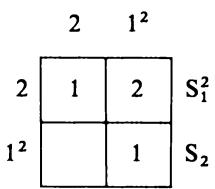
\includegraphics[keepaspectratio]{images/part001_666ab4c0.jpg}}

\pandocbounded{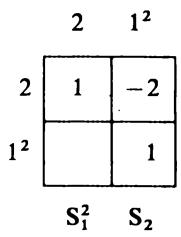
\includegraphics[keepaspectratio]{images/part001_442e375f.jpg}}

\(k = 3\)

3

2.1

\(1^{3}\)

3

1

3

6

\(S_{1}^{3}\)

2.1

1

3

\(S_{1}S_{2}\)

\(1^{3}\)

1

\(S_{3}\)

3 2.1 \(1^{3}\)\\
\pandocbounded{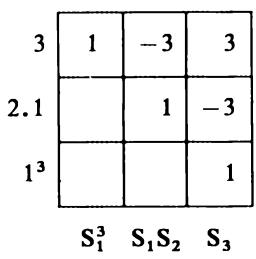
\includegraphics[keepaspectratio]{images/part001_fb1fe29f.jpg}}

\(k = 4\)

4

1

4

6

12

24

\(S_{1}^{4}\)

3.1

1

2

5

12

\(S_{1}^{2}S_{2}\)

\(2^{2}\)

1

2

6

\(S_{2}^{2}\)

\(2.1^{2}\)

1

4

\(S_{1}S_{3}\)

\(1^{4}\)

1

\(S_{4}\)

Matrix C

\pandocbounded{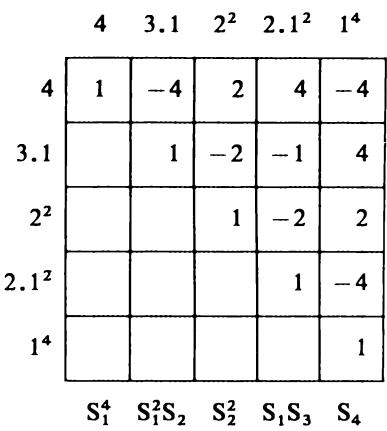
\includegraphics[keepaspectratio]{images/part001_bf35a948.jpg}}

\pandocbounded{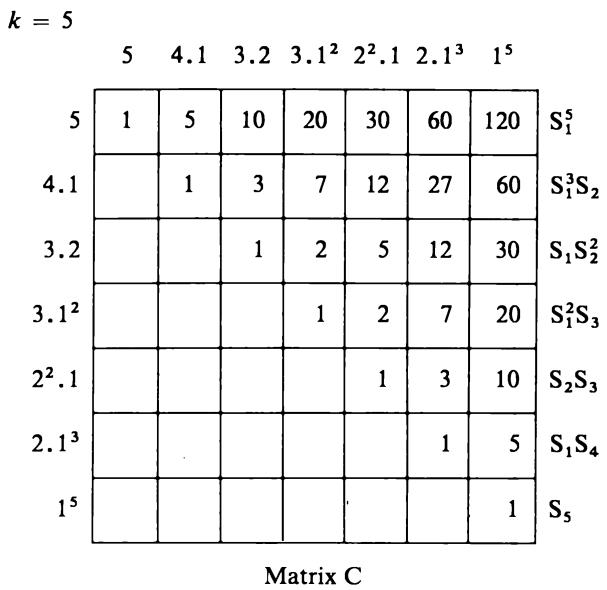
\includegraphics[keepaspectratio]{images/part001_7e862639.jpg}}

\pandocbounded{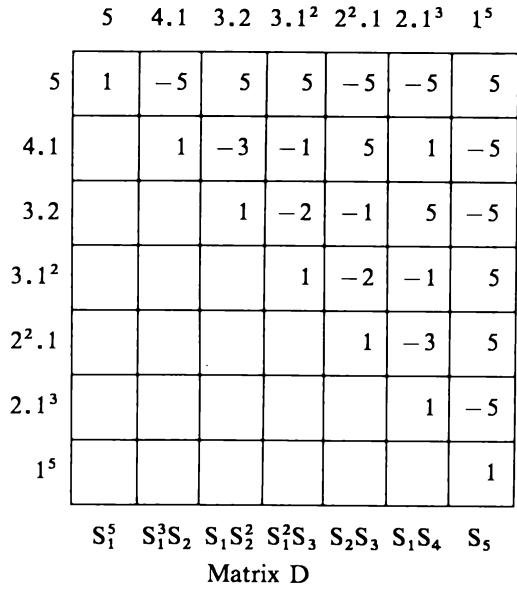
\includegraphics[keepaspectratio]{images/part001_eab66d56.jpg}}


\chapter{Commutative Fields}

Except where the contrary is expressly stated, all the fields considered in this chapter are commutative; all algebras are associative and unital and the algebra homomorphisms are unital, every subalgebra of an algebra contains the unit element of that algebra. Whenever a field K is said to be contained in a ring L (in particular in a field) without further specification, it is understood that K is a subring of L; we shall also say that K is a subfield of L, or also (if L is a field) that L is an extension field of K.

\section{PRIME FIELDS. CHARACTERISTIC}

\subsection{Prime fields}

The field of fractions of the ring Z of rational integers is called the field of rational numbers and is denoted by Q (I, p.~117). For every prime number p the quotient ring \(\mathbf{Z}/(p)\) is a finite \(^{1}\) field of p elements, denoted by \(F_{p}\) in the sequel. The field Q is infinite since it contains Z, and is therefore not isomorphic to any field \(F_{p}\) . If p and \(p'\) are distinct prime numbers, the fields \(F_{p}\) and \(F_{p'}\) have distinct cardinals and so are not isomorphic.

DEFINITION 1. --- A field is said to be prime if it is isomorphic either to Q or to one of the fields \(F_{p}\) .

Every subfield of Q contains the ring Z and hence the field of fractions Q of Z; every subring of \(F_{p}\) is necessarily equal to \(F_{p}\) . Therefore every subfield of a prime field is necessarily equal to it (cf.~Cor. 2 of Th. 1 below). Let P be a prime field and A a ring; if f and \(f'\) are two homomorphisms of P into A, then the set of \(x \in P\) such that \(f(x) = f'(x)\) is a subfield of P, hence by what has been said we must have \(f = f'\) . In particular, the only endomorphism of a prime field is the identity mapping.

THEOREM 1. --- Let A be a ring; suppose that there exists a subfield of A. Then A has a unique subfield P which is a prime field. Moreover, P is contained in the centre of A and in every subfield of A.

Let K be a subfield of A, C the centre of A, and put \(K' = K \cap C\) ; then \(K'\) is a subfield of A. Let f be the unique homomorphism of Z into A and p its kernel. Every subring of A, in particular \(K'\) , contains \(f(\mathbf{Z})\) ; hence the ideal p is prime (I, p.~116-117). If \(\mathfrak{p} = (0)\) , the homomorphism f of Z into \(K'\) is injective; hence it extends (I, p.~116) to an isomorphism \(\bar{f}\) of Q onto a subfield P of \(K'\) . If \(\mathfrak{p} \neq (0)\) , there is a strictly positive integer p such that \(\mathfrak{p} = (p)\) (I, p.~111); if we had p = ab with a \textgreater{} 1 and b \textgreater{} 1, this would mean \(a \notin p\) , \(b \notin p\) and \(ab \in p\) in contradiction with the fact that p is prime. The number p is therefore prime and by passage to quotients f defines an isomorphism of \(F_p = Z/p\) onto a subfield P of \(K'\) . In both cases P is a subfield of A contained in the centre C of A, and it is a prime field. Let L be a subfield of A; then \(P \cap L\) is a subfield of P, and since P is prime, we have \(P \cap L = P\) , whence \(P \subset L\) . If \(P'\) is a subfield of A and is a prime field, then by what has been said, \(P \subset P'\) , whence \(P = P'\) because \(P'\) is a prime field.

COROLLARY 1. --- Let K be a field. There exists a unique subfield of K which is a prime field, and this is the least subfield of K.

COROLLARY 2. --- For a field to be prime it is necessary and sufficient that it should contain no subfield other than itself.

\subsection{Characteristic of a ring and of a field}

We shall define the characteristic of a ring A only when A has a subfield. When this is so, let f be the unique ring homomorphism of Z into A, and let n be the unique positive integer generating the ideal of Z which is the kernel of f (I, p.~111); then the integer n is called the characteristic of A.

Let A be a ring for which the characteristic is defined ; then A does not reduce to 0. By Th. 1 there exists a unique subfield P of A which is a prime field ; we shall call it the prime subfield of A. By the proof of Th. 1 there are the following two possibilities :

\begin{enumerate}
\def\labelenumi{\alph{enumi})}
\item
  the characteristic of A is 0, P is isomorphic to Q,
\item
  the characteristic of \(\mathbf{A}\) is a prime number \(p\) , \(\mathbf{P}\) is isomorphic to \(\mathbf{F}_p\) .
\end{enumerate}

If the characteristic of A is zero, there exists a unique ring homomorphism of Q into A; its image is the prime subfield of A, contained in the centre of A. Therefore there exists a unique Q-algebra structure of A compatible with the ring structure. When the characteristic of A is a prime number p, we have the corresponding properties on replacing the field Q by the field \(F_{p}\) .

PROPOSITION 1. --- Let A be a ring not reduced to 0.

\begin{enumerate}
\def\labelenumi{\alph{enumi})}
\item
  For A to be of characteristic 0 it is necessary and sufficient that the mapping \(x \mapsto n \cdot x\) of A into itself should be bijective, for every integer \(n \neq 0\) .
\item
  Let \(p\) be a prime number. For \(\mathbf{A}\) to be of characteristic \(p\) it is necessary and sufficient that \(p \cdot x = 0\) for all \(x \in \mathbf{A}\) .
\end{enumerate}

Let \(f\) be the unique homomorphism of \(\mathbf{Z}\) into \(\mathbf{A}\) ; we have \(n \cdot x = f(n)x\) for every integer \(n\) and every \(x\) in \(\mathbf{A}\) . For \(\mathbf{A}\) to be of characteristic 0, it is necessary and sufficient that \(f\) should extend to a homomorphism of \(\mathbf{Q}\) into \(\mathbf{A}\) , that is, \(f(n)\) should be invertible in \(\mathbf{A}\) for every \(n \neq 0\) (I, p.~113); this proves \(a\) ). Similarly for \(\mathbf{A}\) to be of characteristic \(p\) it is necessary and sufficient that \(f\) should annihilate \(p\mathbf{Z}\) , that is, \(f(p) = 0\) , or also that \(p \cdot x = 0\) for all \(x \in \mathbf{A}\) ; this proves \(b\) .

Let us take for A a not necessarily commutative field. The centre of A is a (commutative) field; therefore the characteristic and the prime subfield of A are defined.

Remarks. --- 1) Let A and A' be two rings not reduced to 0. Suppose that the characteristic of A is defined and that there is a homomorphism u of A into A'. The image under u of the prime subfield of A is a subfield P' of A', isomorphic to P, and hence prime. It follows that the characteristic of A' is defined and is equal to that of A. If A and A' are of characteristic 0 (resp. \(p \neq 0\) ), the mapping u is a homomorphism of algebras over Q (resp. \(F_{p}\) ).

\begin{enumerate}
\def\labelenumi{\arabic{enumi})}
\setcounter{enumi}{1}
\item
  Remark 1 shows that if A is a ring of characteristic 0 (resp. \(p \neq 0\) ), the same holds of any ring A' containing A as subring, or of any quotient of A by a two-sided ideal \(\mathfrak{a} \neq \mathbf{A}\) . In particular, if K is a field, every subfield of K and every extension field of K have the same characteristic as K.
\item
  Let A be an algebra not reduced to 0 over a field K. Since the mapping \(\lambda \mapsto \lambda \cdot 1\) of K into A is a ring homomorphism, Remark 1 shows that the characteristic of A is defined and equal to that of K.
\item
  Since the field \(\mathbf{Q}\) is infinite, every ring of characteristic 0 is infinite; it follows that every finite field has non-zero characteristic.
\item
  Let A be a ring not reduced to 0, whose additive group is a torsion-free Z-module, and put \(B = Q \otimes_{Z} A\) . The mapping \(x \mapsto 1 \otimes x\) of A into B is injective (II, p.~314), hence A is isomorphic to a subring of a ring of characteristic 0.
\end{enumerate}

\subsection{\texorpdfstring{Commutative rings of characteristic \(p\)}{Commutative rings of characteristic p}}

In this No.~and the following one p denotes a prime number.

THEOREM 2. --- Let A be a commutative ring of characteristic p.~The mapping \(a \mapsto a^{p}\) is an endomorphism of the ring A, that is, we have the relations

\[
(a + b) ^ {p} = a ^ {p} + b ^ {p}\tag{1}
\]

\[
(a b) ^ {p} = a ^ {p} b ^ {p}\tag{2}
\]

for \(a, b\) in A.

Formula (2) follows from the commutativity of A. To prove (1) we use the binomial formula \((a + b)^p = a^p + b^p + \sum_{i=1}^{p-1} \binom{p}{i} \cdot a^ib^{p-i}\) ; since \(p \cdot x = 0\) for all \(x \in \mathbf{A}\) , it suffices to prove the following lemma:

Lemma 1. --- Let \(p\) be a prime number and \(i\) an integer in the range from 1 to \(p - 1\) , then the binomial coefficient \(\binom{p}{i}\) is an integer divisible by \(p\) .

We argue by induction on \(i\) , the case \(i = 1\) being immediate from the formula \(\binom{p}{1} = p\) . Suppose that \(2 \leqslant i \leqslant p - 1\) and that \(\binom{p}{i - 1}\) is divisible by \(p\) . Then the integer \(i\binom{p}{i} = (p - i + 1)\binom{p}{i - 1}\) belongs to the prime ideal \(p\mathbf{Z}\) of \(\mathbf{Z}\) ; since \(i \notin p\mathbf{Z}\) , we have \(\binom{p}{i} \in p\mathbf{Z}\) and the lemma follows.

Let A be a commutative ring of characteristic p and f an integer \(\geqslant0\) . From Th. 2 we deduce by induction on f that the mapping \(a\mapsto a^{p^{f}}\) is an endomorphism of the ring A. In particular we have the relation

\[
(a _ {1} + \dots + a _ {n}) ^ {p ^ {f}} = a _ {1} ^ {p ^ {f}} + \dots + a _ {n} ^ {p ^ {f}}\tag{3}
\]

for any \(a_{1},\ldots,a_{n}\) in A. The mapping \(a\mapsto a^{p}\) is sometimes called the Frobenius endomorphism of A. Taking \(\mathbf{A}=\mathbf{F}_{p}\) and \(a_{i}=1\) , we obtain from (3) the relation:

\[
n ^ {p ^ {f}} \equiv n \mod p (n \in \mathbf {Z}, f \in \mathbf {N}).\tag{4}
\]

For each subset S of A we denote by \(S^{p^{f}}\) the set of elements of A of the form \(x^{p^{f}}\) with \(x \in S\) \(^{1}\) . In particular, if K is a subring of A, the set \(K^{p^{f}}\) is a subring of A. If K is a subring of A and S a subset of A we denote by K{[}S{]} the subring of A generated by \(K \cup S\) ; when A is a field, we denote by \(\mathrm{K}(S)\) the field of fractions of K{[}S{]}, that is, the subfield of A generated by \(K \cup S\) .

PROPOSITION 2. --- Let A be a commutative ring of characteristic p, K a subring of A, S a subset of A and f a positive integer.

\begin{enumerate}
\def\labelenumi{\alph{enumi})}
\item
  We have \(\mathbf{K}[\mathbf{S}]^{p^f} = \mathbf{K}^{p^f}[\mathbf{S}^{p^f}]\) , and if \(\mathbf{A}\) is a field, \(\mathbf{K}(\mathbf{S})^{p^f} = \mathbf{K}^{p^f}(\mathbf{S}^{p^f})\) .
\item
  If the K-module K{[}S{]} is generated by the family \((a_{i})_{i\in I}\) of elements of A, then the K-module \(K[S^{p^{f}}]\) is generated by the family \((a_{i}^{p^{f}})_{i\in I}\) .
\end{enumerate}

Since K{[}S{]} is the subring of A generated by K ∪ S, its image K{[}S{]} \(^{p^{f}}\) under the endomorphism \(\pi: a \mapsto a^{p^{f}}\) of the ring A is the subring of A generated by the image K \(^{p^{f}}\) ∪ S \(^{p^{f}}\) of K ∪ S under \(\pi\) , whence K{[}S{]} \(^{p^{f}}\) = K \(^{p^{f}}\) {[}S \(^{p^{f}}\) {]}. The case of fields is treated similarly; this proves a).

It is clear that the family \((a_i^{p^f})_{i\in I}\) generates the \(\mathbf{K}^{p^f}\) -module \(\mathbf{K}[\mathbf{S}]^{p^f}\) . The K-module \(\mathbf{K}[\mathbf{S}^{p^f}]\) is generated by products of the form \(x_1^{p^f}\ldots x_n^{p^f} = (x_1\ldots x_n)^{p^f}\) with \(x_1,\ldots ,x_n\) arbitrary in S, hence also by the set \(\mathbf{K}[\mathbf{S}]^{p^f}\) . Assertion b) follows directly from this.

\(^{1}\) Of course the set \(S^{p^{f}}\) should not be confused with the set product of \(p^{f}\) sets equal to S, nor with the set of products of \(p^{f}\) elements belonging to S.

\subsection{\texorpdfstring{Perfect rings of characteristic \(p\)}{Perfect rings of characteristic p}}

DEFINITION 2. --- A ring A of characteristic \(p \neq 0\) is said to be perfect if it is commutative and the mapping \(a \mapsto a^p\) is bijective.

If the ring A is perfect of characteristic p, the mapping \(a \mapsto a^{p^{f}}\) is an automorphism of the ring A for every integer \(f \geqslant 0\) ; the inverse automorphism is denoted by \(a \mapsto a^{1/p^{f}}\) or \(a \mapsto a^{p^{-f}}\) and the image of a subset S of A under this automorphism is written \(S^{1/p^{f}}\) or \(S^{p^{-f}}\) . It is clear that \((a^{p^{e}})^{p^{f}} = a^{p^{e+f}}\) for all \(a \in A\) and any integers e and f (of whatever sign).

Let A be a commutative ring of characteristic p.~For every integer \(f \geqslant 0\) let us write \(n_{f}\) for the kernel of the endomorphism \(a \mapsto a^{p^{f}}\) of the ring A. Then \((\mathfrak{n}_{f})_{f \geqslant 0}\) is an increasing sequence of ideals of A; since every positive integer is majorized by a power of p, the ideal \(n = \bigcup_{f \geqslant 0} n_{f}\) consists of all the

nilpotent elements of A. In particular, if A is perfect, every nilpotent element of A is zero.

DEFINITION 3. --- Let A be a commutative ring of characteristic \(p \neq 0\) . By a perfect closure of A we understand a pair \((\hat{\mathbf{A}}, u)\) where \(\hat{\mathbf{A}}\) is a perfect ring of characteristic \(p\) and \(u\) is a homomorphism of A into \(\hat{\mathbf{A}}\) satisfying the following universal property:

(PC) If B is a perfect ring of characteristic p and v is a homomorphism of A into B, then there exists a unique homomorphism h of \(\hat{A}\) into B such that \(v = h \circ u\) .

The universal property (PC) implies at once the uniqueness of the perfect closure, in the following sense: if \((\hat{\mathbf{A}}, u)\) and \((\hat{\mathbf{A}}', u')\) are two perfect closures of A, then there exists a unique isomorphism h of \(\hat{A}\) onto \(\hat{A}'\) such that \(u' = h \circ u\) (cf.~E, IV, p.~23). We shall now establish the existence of the perfect closure:

THEOREM 3. --- Let A be a commutative ring of characteristic \(p \neq 0\) . There exists a perfect closure \((\hat{\mathbf{A}}, u)\) of A. Moreover, the kernel of \(u\) is the set of all nilpotent elements of A and for each \(x \in \hat{\mathbf{A}}\) there exists an integer \(n \geqslant 0\) such that \(x^{p^n} \in u(\mathbf{A})\) .

For each integer \(n \geqslant 0\) , put \(\mathbf{A}_n = \mathbf{A}\) ; when \(m \geqslant n\) we define a homomorphism \(\pi_{m,n}\) of \(\mathbf{A}_n\) into \(\mathbf{A}_m\) by \(\pi_{m,n}(a) = a^{p^{m-n}}\) . We thus obtain a direct system of rings \((\mathbf{A}_n, \pi_{m,n})\) (I, p.~120); let \(\hat{\mathbf{A}}\) be the direct limit of this system and \(u_n\) the canonical homomorphism of \(\mathbf{A}_n = \mathbf{A}\) into \(\hat{\mathbf{A}}\) ; we also put \(u = u_0\) . By construction of the direct limit the kernel \(n\) of \(u\) is the union of the kernels of the homomorphisms \(\pi_{n,0}: a \mapsto a^{p^n}\) of A into A, thus it consists of all the nilpotent elements of A. The ring \(\hat{A}\) is commutative of characteristic p by Remark 1 of V, p.~3.

The ring \(\hat{\mathbf{A}}\) is the union of the ascending sequence \((u_n(\mathbf{A}))_{n\geq 0}\) of subrings. We have \(u_{n}(\mathbf{A})^{p^{n}} = \mathbf{A}\) ; hence for each \(x\in \hat{\mathbf{A}}\) there exists an integer \(n\geqslant 0\) such that \(x^{p^n}\in u(\mathbf{A})\) . We also have \(u_{n}(\mathbf{A}) = u_{n + 1}(\mathbf{A})^{p}\) , whence \(\hat{\mathbf{A}}^p = \hat{\mathbf{A}}\) . Let \(x\in \hat{\mathbf{A}}\) be such that \(x^{p} = 0\) ; choose an integer \(n\geqslant 1\) and an element \(a\in \mathbf{A}\) such that \(x = u_{n}(a)\) . Then we have \(u_{n - 1}(a) = u_n(a)^p = 0\) ; by definition of the direct limit there exists an integer \(m\geqslant n\) such that \(\pi_{m - 1,n - 1}(a) = 0\) , that is, \(a^{p^{m - n}} = 0\) . We thus have \(\pi_{m,n}(a) = 0\) , whence \(u_{n}(a) = 0\) , that is, \(x = 0\) . Therefore the ring \(\hat{\mathbf{A}}\) is perfect of characteristic \(p\) .

Let \(v\) be a homomorphism of \(A\) into a perfect ring \(B\) of characteristic \(p\) . For every integer \(n \geqslant 0\) , the mapping \(b \mapsto b^{p^n}\) is an automorphism of \(B\) and so there exists a homomorphism \(v_n\) of \(A_n = A\) into \(B\) characterized by \(v(a) = v_n(a)^{p^n}\) . We then have \(v_m \circ \pi_{m,n} = v_n\) for \(m \geqslant n \geqslant 0\) ; by definition of the direct limit there exists a homomorphism \(h\) of \(\hat{A}\) into \(B\) such that \(v_n = h \circ u_n\) for all \(n \geqslant 0\) ; in particular we have \(v = v_0 = h \circ u_0 = h \circ u\) . Finally let \(h'\) be a homomorphism of \(\hat{A}\) into \(B\) such that \(h' \circ u = v\) . Let \(x \in \hat{A}\) ; as we have seen, there exist an integer \(n \geqslant 0\) and an element \(a \in A\) such that \(x^{p^n} = u(a)\) . Then we have

\[
h (x) ^ {p ^ {n}} = h (u (a)) = v (a) = h ^ {\prime} (u (a)) = h ^ {\prime} (x) ^ {p ^ {n}},
\]

and since B is perfect, we find \(h(x) = h'(x)\) . Thus we have \(h' = h\) , and this completes the proof that \((\hat{\mathbf{A}}, u)\) is a perfect closure of A.

PROPOSITION 3. --- Let B be a perfect ring of characteristic p and A a subring of B. Write \(A^{p^{-\infty}} = \bigcup_{f \geqslant 0} A^{p^{-f}}\) and denote by j the canonical injection of A in

\(\mathbf{A}^{p^{-\infty}}\) . Then \(\mathbf{A}^{p^{-\infty}}\) is the smallest perfect subring of \(\mathbf{B}\) containing \(\mathbf{A}\) and \((\mathbf{A}^{p^{-\infty}}, j)\) is a perfect closure of \(\mathbf{A}\) .

For each integer \(f \in \mathbf{Z}\) denote by \(\pi_f\) the automorphism \(b \mapsto b^{p^f}\) of \(\mathbf{B}\) . The sequence of subrings \(\pi_{-f}(\mathbf{A})\) of \(\mathbf{B}\) (for \(f \geqslant 0\) ) is ascending and its union \(\mathbf{A}^{p^{-\infty}}\) is thus a subring of \(\mathbf{B}\) . We have \(\pi_1(\mathbf{A}^{p^{-\infty}}) = \bigcup_{f \geqslant 0} \pi_{-(f-1)}(\mathbf{A}) = \mathbf{A}^{p^{-\infty}}\) , hence

\(A^{p^{-\infty}}\) is a perfect subring of B. Finally let \(B_0\) be a perfect subring of B containing A; for every integer \(f \geqslant 0\) we have \(\pi_{-f}(A) \subset \pi_{-f}(B_0) = B_0\) , whence \(A^{p^{-\infty}} \subset B_0\) .

If \(v\) is a homomorphism of \(\mathbf{A}\) into a perfect ring \(\mathbf{B}'\) of characteristic \(p\) , then for every integer \(f \geqslant 0\) we can define a homomorphism \(h_f\) of \(\pi_{-f}(\mathbf{A})\) into \(\mathbf{B}'\) by \(h_f(\pi_{-f}(a)) = v(a)^{p^{-f}}\) for all \(a \in \mathbf{A}\) . We see at once that \(h_{f + 1}\) agrees with \(h_f\) on \(\pi_{-f}(\mathbf{A})\) ; thus there exists a homomorphism \(h\) of \(\mathbf{A}^{p^{-\infty}}\) into \(\mathbf{B}'\) which induces \(h_f\) on \(\pi_{-f}(\mathbf{A})\) for all \(f \geqslant 0\) and in particular, \(h\) extends \(h_0 = v\) . If \(h'\) is another extension of v to a homomorphism of \(A^{p^{-\infty}}\) into B, the equality \(h' = h\) may be established as in the proof of Th. 3.

\subsection{Characteristic exponent of a field. Perfect fields}

Let K be a field. By the characteristic exponent of K we understand the integer equal to 1 if K is of characteristic 0, and equal to the characteristic of K when this is non-zero.

PROPOSITION 4. --- Let K be a field of characteristic exponent q. For every integer \(f \geqslant 0\) the mapping \(x \mapsto x^{q^{f}}\) is an isomorphism of K on one of its subfields (denoted by \(K^{q^{f}}\) ).

This follows from Th. 2 when \(q \neq 1\) and is trivial when \(q = 1\) .

Likewise one can extend Prop. 2 to the case where A is a field of characteristic exponent q, the case q = 1 being trivial.

DEFINITION 4. --- A field K of characteristic exponent q is said to be perfect if we have \(K^{q} = K\) . When \(K^{q} \neq K\) , K is called imperfect.

By this definition a field is perfect if it is of characteristic 0, or if it is a perfect ring of characteristic \(p \neq 0\) in the sense of Def. 2. If \(\mathbf{K}\) is a field of characteristic \(p \neq 0\) and \((\hat{\mathbf{K}}, u)\) is a perfect closure of \(\mathbf{K}\) , then \(\hat{\mathbf{K}}\) is a field by Prop. 3 (V, p.~6) and \(u\) is an isomorphism of \(\mathbf{K}\) onto a subfield of \(\hat{\mathbf{K}}\) . Frequently one identifies \(\mathbf{K}\) with its image under \(u\) in \(\hat{\mathbf{K}}\) , so that we have \(\hat{\mathbf{K}} = \mathbf{K}^{p^{-\infty}}\) (Prop. 3).

Let K be a field of characteristic 0; the characteristic exponent of K is then 1. By convention the notation \(x^{q^{-f}}\) and \(S^{q^{-f}}\) is taken to mean x and S respectively (for an element x of K and a subset S of K). In particular we put \(K^{q^{-\infty}} = K\) and we agree to take the perfect closure of K to be K.

PROPOSITION 5. --- If K is a field of characteristic 0, or is finite, * or algebraically closed *, it is perfect. In particular every prime field is perfect.

Suppose that K has characteristic \(p \neq 0\) . If K is finite, then the subfield \(K^{p}\) of K has the same cardinal as K, whence \(K^{p} = K\) . * If K is algebraically closed, the polynomial \(X^{p} - a\) has a root x in K for each \(a \in K\) (V, p.~20, Def. 1) whence \(x^{p} = a\) and so \(K^{p} = K\) . * Finally a prime field is of characteristic 0 or finite.

Let \(K_{0}\) be a field of characteristic \(p \neq 0\) and \(\mathbf{K} = \mathbf{K}_{0}(\mathbf{X})\) the field of rational fractions in an indeterminate X over \(K_{0}\) . Then K is imperfect, for there exists no element \(u(\mathbf{X})/v(\mathbf{X})\) of K (u, v polynomials in \(K_{0}[\mathbf{X}]\) ) such that \((u(\mathbf{X})/v(\mathbf{X}))^{p} = \mathbf{X}\) . This may be seen by writing this relation in the form \(u(\mathbf{X})^{p} = \mathbf{X}v(\mathbf{X})^{p}\) and comparing the degrees of the two sides.

\subsection{Characterization of polynomials with zero differential}

PROPOSITION 6. --- Let K be a commutative ring, A the polynomial algebra \(K[X_{i}]_{i \in I}\) and S the set of elements F of A such that dF = 0.

\begin{enumerate}
\def\labelenumi{\alph{enumi})}
\item
  If \(\mathbf{K}\) is a ring of characteristic 0, then \(\mathbf{S} = \mathbf{K}\) .
\item
  If \(\mathbf{K}\) is a ring of characteristic \(p \neq 0\) , then \(\mathbf{S} = \mathbf{K}[\mathbf{X}_i^p]_{i \in I}\) ; if moreover \(\mathbf{K}\) is perfect, then \(\mathbf{K} = \mathbf{A}^p\) .
\end{enumerate}

The mapping \(F \mapsto dF\) of A into the module \(\Omega_{\mathbf{K}}(\mathbf{A})\) of K-differentials of A is K-linear and satisfies the relation

\[
d \left(\mathrm{FF} ^ {\prime}\right) = \mathrm{F} \cdot d \mathrm{F} ^ {\prime} + \mathrm{F} ^ {\prime} \cdot d \mathrm{F}
\]

(III, p.~569). Therefore S is a subalgebra.

When K is of characteristic \(p \neq 0\) , put \(T = K[X_{i}^{p}]_{i \in I}\) ; we thus have \(T = A^{p}\) if K is perfect (V, p.~4, Prop. 2); moreover, we have \(d(X_{i}^{p}) = pX_{i}^{p-1}\) . \(dX_{i} = 0\) for all \(i \in I\) , hence the subalgebra S of A contains T. If K is of characteristic 0, we put T = K, and still find that \(T \subset S\) . It remains to show that S is contained in T.

For every finite subset \(J\) of \(I\) let \(A_{J}\) be the subalgebra of \(A\) generated by the family \((X_{j})_{j\in J}\) . We have \(A_{\emptyset} = K\) and \(A = \bigcup_{J\in I}A_{J}\) ; so it suffices to prove the

relation \(S \cap A_{J} \subset T\) , which we shall accomplish by induction on the cardinal of J. Thus let J be a finite subset of I such that \(S \cap A_{J} \subset T\) , let i be an element of I - J and \(J' = J \cup \{i\}\) . Every element F of \(A_{J}\) may be written in just one way in the form

\[
\mathrm{F} = \sum_ {n = 0} ^ {\infty} \mathrm{F} _ {n} \cdot \mathrm{X} _ {i} ^ {n},\tag{5}
\]

with \(\mathbf{F}_n\in \mathbf{A}_{\mathrm{J}}\) for all \(n\geqslant 0\) , and then

\[
d \mathrm{F} = \sum_ {n = 0} ^ {\infty} \mathrm{X} _ {i} ^ {n} \cdot d \mathrm{F} _ {n} + \sum_ {n = 0} ^ {\infty} n \mathrm{X} _ {i} ^ {n - 1} \mathrm{F} _ {n} \cdot d \mathrm{X} _ {i}.\tag{6}
\]

Suppose that F belongs to S; the family \((d\mathbf{X}_{r})_{r\in I}\) is a basis of the A-module \(\Omega_{\mathrm{K}}(\mathbf{A})\) (III, p.~570) and \(dF_{n}\) is a linear combination of the differentials \(dX_{j}\) for \(j\in J\) because \(F_{n}\in A_{J}=K[X_{j}]_{j\in J}\) . By (6) we then have \(dF_{n}=0\) and \(nF_{n}=0\) for each integer \(n\geqslant0\) . By the induction hypothesis \(F_{n}\in T\) for all n, since \(dF_{n}=0\) .

\begin{enumerate}
\def\labelenumi{\alph{enumi})}
\item
  If K is of characteristic 0, we have \(nF_{n} = 0\) for all \(n \geqslant 1\) , whence \(F_{n} = 0\) by Prop. 1 (V, p.~2); so we have \(F = F_{0}\) , whence \(F \in T\) .
\item
  If \(\mathbf{K}\) is of characteristic \(p \neq 0\) , then \(\mathbf{A}\) is an algebra over the field \(\mathbf{F}_p\) and the relation \(n\mathrm{F}_n = 0\) implies \(\mathbf{F}_n = 0\) for every integer \(n\) not divisible by \(p\) . So we have \(\mathbf{F} = \sum_{m=0}^{\infty} \mathbf{F}_{mp} \mathbf{X}_i^{mp}\) , whence \(\mathbf{F} \in \mathbf{T}\) .
\end{enumerate}

Remark. --- We still have S = K when the additive group of K is torsion-free; this follows from the above proof or from Remark 5 of V, p.~3.

COROLLARY. --- Let K be a field and F(X) a polynomial with coefficients in K, whose derivative F'(X) is zero.

\begin{enumerate}
\def\labelenumi{\alph{enumi})}
\item
  If \(\mathbf{K}\) is of characteristic 0, then \(\mathbf{F} \in \mathbf{K}\) .
\item
  If \(\mathbf{K}\) is of characteristic \(p \neq 0\) , there exists a polynomial \(\mathbf{G}(\mathbf{X})\) such that \(\mathbf{F}(\mathbf{X}) = \mathbf{G}(\mathbf{X}^p)\) .
\end{enumerate}

For we have \(d\mathbf{F} = \mathbf{F}' \cdot d\mathbf{X} = 0\) .

\section{EXTENSIONS}

\subsection{The structure of an extension}

DEFINITION 1. --- Let K be a field. By an extension of K we understand a K-algebra whose underlying ring is a field. By a subextension (or sub-K-extension) of the extension E we understand a sub-K-algebra of E which is a field.

Let E be an extension of K. The mapping \(u: \lambda \mapsto \lambda \cdot 1\) of K into E is a ring homomorphism; by I, p.~115, u induces an isomorphism of K onto a subfield \(u(\mathbf{K})\) of E.

Conversely, if K, E are fields and u is a homomorphism of K into E, then u defines on E a structure of extension of K (III, p.~433). By abuse of language one sometimes says that \((E, u)\) is an extension of K.

An extension is said to be trivial if \(u(\mathbf{K}) = \mathbf{E}\) , that is, if E is a vector space of dimension 1 over K.

Let L be an extension field of K. When we consider L as extension of K, we understand by this the extension \((L, j)\) of K, where j is the canonical injection of K into L, or also L with the corresponding K-algebra structure. The subextensions of L are then the intermediate fields between K and L, that is, the subfields of L containing K. If \(L'\) is another extension field of K, a K-homomorphism of L into \(L'\) is then a homomorphism f of L into \(L'\) such that \(f(x) = x\) for all \(x \in K\) . We note that if f is any endomorphism of the field L, then the set of elements of L invariant under f is a subfield \(K'\) of L, and that f is then a \(K'\) -endomorphism of L.

In particular let P be the prime subfield of a field L. We can consider L as an extension of P, and every endomorphism of L is then a P-endomorphism.

\pandocbounded{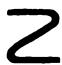
\includegraphics[keepaspectratio]{images/part001_5fd131d7.jpg}}

Let \((\mathrm{E}, u)\) be an extension of K; since u defines an isomorphism of K onto a subfield \(K_{1}\) of E, there is in general no difficulty in identifying K with \(K_{1}\) by means of u. One case where we cannot allow such an identification is that where K = E and where u is thus an endomorphism of K; most frequently u will be an automorphism of K, or the mapping \(u \mapsto u^{p}\) , when the field K is of characteristic \(\neq 0\) .

It is clear that every extension of K is isomorphic to an extension \((L, j)\) , where L is a field containing K as subfield and j is the canonical injection of K into L.

\subsection{Degree of an extension}

Let A be an algebra over a field K. It is in particular a vector space over K; the dimension of this vector space is called the degree of A over K and is written \([A:K]\) (II, p.~293). By definition \([A:K]\) is thus the cardinal of any basis of A over K. This definition applies in particular to the case of extensions of K.

An extension of degree 1 is trivial. An extension of degree 2 (resp. 3 etc.) is called quadratic (resp. cubic etc.). An extension of finite degree is sometimes called, by abuse of language, a finite extension.

THEOREM 1. --- Let E be an extension of K and A an algebra over E. Then we have \([A:K]=[A:E]\) . \([E:K]\) . In particular, if F is an extension of E, we have

\[
[ \mathbf {F}: \mathbf {K} ] = [ \mathbf {F}: \mathbf {E} ]. [ \mathbf {E}: \mathbf {K} ].\tag{1}
\]

The theorem is just a special case of II, p.~222, Prop. 25; more precisely, if \((a_{\lambda})_{\lambda \in L}\) is a basis of A over E and \((b_{\mu})_{\mu \in M}\) a basis of E over K, then the family \((a_{\lambda}b_{\mu})_{(\lambda ,\mu)\in L\times M}\) is a basis of A over K.

COROLLARY 1. --- Let K, E, F be three fields such that \(K \subset E \subset F\) and \([F:K]\) is finite. Then the degrees \([E:K]\) and \([F:E]\) are divisors of \([F:K]\) .

If the degree \([F:K]\) is prime, there is thus no subextension of F other than K and F. But note that when \([F:K]\) is not prime, there is not necessarily a subextension of F other than K and F (cf.~V, p.~146, Exercise 1).

COROLLARY 2. --- Let K, E and F be three fields such that \(K \subset E \subset F\) . Suppose that \([F:K]\) is finite, then the relation \([E:K] = [F:K]\) is equivalent to E = F and the relation \([F:E] = [F:K]\) is equivalent to E = K.

For if L is an extension field of \(L'\) then \([L:L'] = 1\) is equivalent to \(L' = L\) .

PROPOSITION 1. --- Let A be an algebra of finite degree over a field K. If an element \(a \in \mathbf{A}\) is not a left (resp. right) divisor of zero in A, then it is invertible in A.

For the vector space A over K is of finite dimension, by hypothesis, and the linear mapping \(x \mapsto ax\) (resp. \(x \mapsto xa\) ) of A into A is injective; it is therefore bijective (II, p.~298, Cor.) and hence (I, p.~16, Remark) a is invertible in A.

COROLLARY. --- Let A be a commutative algebra of finite degree over a field K. If A is an integral domain, then it is a field.

\subsection{Adjunction}

Let E be an extension of a field K. Given a family \(\mathbf{x} = (x_{i})_{i \in I}\) of elements of E, we denote by \(\mathrm{K}(x_{i})_{i \in I}\) (or \(\mathrm{K}(\mathbf{x})\) or also \(\mathrm{K}(x_{1}, \ldots, x_{n})\) when I is the interval {[}1, n{]} of N) the least subextension of E containing the members of the family \((x_{i})\) ; we say that \(\mathrm{K}(x_{i})_{i\in I}\) is obtained by adjunction to K of the elements of the family \((x_{i})_{i\in I}\) and that the family \((x_{i})_{i\in I}\) (or the set of its elements) is a generating family of \(\mathrm{K}(x_{i})_{i\in I}\) with respect to K (or over K). The field \(\mathrm{K}(x_{i})_{i\in I}\) depends only on the set A of elements of the family \((x_{i})_{i\in I}\) ; we also denote it by \(\mathrm{K}(\mathrm{A})\) . In particular we have \(\mathrm{K}(\mathrm{E})=\mathrm{E}\) and \(\mathrm{K}(\emptyset)=\mathrm{K} \cdot 1\) . All that has been said applies in particular when E is a field containing K as subfield.

\pandocbounded{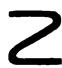
\includegraphics[keepaspectratio]{images/part001_724f36f3.jpg}}

It should be observed that A is not in general a generating set of the algebra \(\mathbf{K}(\mathbf{A})\) , in other words that \(\mathbf{K}(\mathbf{A}) \neq \mathbf{K}[\mathbf{A}]\) . * Nevertheless we shall see that \(\mathbf{K}(\mathbf{A}) = \mathbf{K}[\mathbf{A}]\) when \(\mathbf{K}(\mathbf{A})\) is an algebraic extension of \(\mathbf{K}\) (V, p.~18, Cor. 1) . *

PROPOSITION 2. --- If M and N are any two subsets of an extension of a field K, then \(\mathbf{K}(\mathbf{M} \cup \mathbf{N}) = \mathbf{K}(\mathbf{M})(\mathbf{N}) = \mathbf{K}(\mathbf{N})(\mathbf{M})\) .

For \(\mathbf{K}(\mathbf{M} \cup \mathbf{N})\) contains \(\mathbf{K}(\mathbf{M})\) and \(\mathbf{N}\) and hence \(\mathbf{K}(\mathbf{M})(\mathbf{N})\) ; since \(\mathbf{K}(\mathbf{M})(\mathbf{N})\) is a field containing \(\mathbf{K} \cup \mathbf{M} \cup \mathbf{N}\) , it contains \(\mathbf{K}(\mathbf{M} \cup \mathbf{N})\) , whence the proposition.

We shall sometimes write \(\mathbf{K}(\mathbf{M},\mathbf{N})\) instead of \(\mathbf{K}(\mathbf{M}\cup \mathbf{N})\) .

Remark. --- Let P be the prime subfield of a field E (V, p.~2) ; for every subset A of E, P(A) is the least subfield of E containing A. In particular if K is a subfield of E, we have P(K ∪ A) = K(A). If K and K' are two subfields of E, we thus have P(K ∪ K') = K(K') = K'(K) ; this field is the least subfield of E containing K or K', or also the upper bound of K and K' in the set of subfields of E, ordered by inclusion ; we sometimes say that this field is the field generated by K and K' in E.

PROPOSITION 3. --- Let F be a set of subfields of a field E, directed with respect to the relation ⊂. The union L of the fields of F is a field.

For if \(x\) and \(y\) are two elements of \(L\) , there exist two fields \(R, S\) of \(\mathcal{F}\) such that \(x \in R\) , \(y \in S\) ; let \(T\) be a field of \(\mathcal{F}\) containing \(R\) and \(S\) ; then \(x \in T\) , \(y \in T\) , hence \(x + y\) , \(xy\) and \(x^{-1}\) (if \(x \neq 0\) ) belong to \(T\) , hence to \(L\) .

COROLLARY. --- Let E be an extension of a field K and A ⊂ E. The field K(A) is the union of the fields K(F) where F ranges over the set of all finite subsets of A.

For the set of fields \(\mathbf{K}(\mathbf{F})\) is directed by the relation \(\subset\) , because \(F \subset F'\) implies \(\mathbf{K}(\mathbf{F}) \subset \mathbf{K}(\mathbf{F}')\) . The union L of these fields is thus a field containing \(K \cup A\) and contained in \(\mathbf{K}(\mathbf{A})\) , and hence identical with \(\mathbf{K}(\mathbf{A})\) .

DEFINITION 2. --- An extension E of a field K is said to be finitely generated if it has a finite generating family. It is called monogenous if there exists x in E such that \(E = K(x)\) .

\pandocbounded{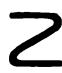
\includegraphics[keepaspectratio]{images/part001_c96515a7.jpg}}

The Cor. of Prop. 3 shows that every extension E of a field K is a directed union of finitely generated extensions contained in E. It is clear that every extension E of K of finite degree is also finitely generated because a basis of E (considered as vector space over K) is also a generating family of E over K; we shall see later that the converse does not hold.

\subsection{Composite extensions}

Let E and F be two extensions of a field K. By a composite extension of E and F we understand any triple \((L, u, v)\) , where L is an extension of K, u is a K-homomorphism of E into L and v is a K-homomorphism of F into L, and where the field L is generated by \(u(E) \cup v(F)\) (cf.~Fig. 1).

\pandocbounded{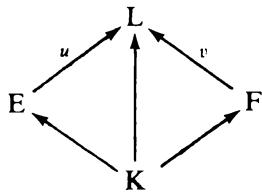
\includegraphics[keepaspectratio]{images/part001_6a404f81.jpg}}\\
FIG. 1.

In agreement with the general definitions (E, IV, p.~6) an isomorphism of a composite extension \((L, u, v)\) of E and F onto a composite extension \((L', u', v')\) of E and F is a K-isomorphism \(\varphi\) of L onto \(L'\) such that \(u' = \varphi \circ u\) and \(v' = \varphi \circ v\) .

Let \((\mathbf{L}, u, v)\) be a composite extension of \(\mathbf{E}\) and \(\mathbf{F}\) . The K-linear mapping \(w\) of \(\mathbf{E} \otimes_{\mathbf{K}} \mathbf{F}\) into \(\mathbf{L}\) which sends \(x \otimes y\) to \(u(x)v(y)\) is a K-algebra homomorphism; in this No.~we shall denote it by \(u * v\) . Its image is the subring of \(\mathbf{L}\) generated by \(u(\mathbf{E}) \cup v(\mathbf{F})\) .

PROPOSITION 4. --- Let E, F be two extensions of K.

\begin{enumerate}
\def\labelenumi{\alph{enumi})}
\item
  Let \((\mathbf{L}, u, v)\) be a composite extension of \(\mathbf{E}\) and \(\mathbf{F}\) ; then the kernel \(\mathfrak{p}\) of the homomorphism \(u * v\) of \(\mathbf{E} \otimes_{\mathbf{K}} \mathbf{F}\) into \(\mathbf{L}\) is a prime ideal.
\item
  Let \(\mathfrak{p}\) be a prime ideal of \(E \otimes_{K} F\) ; then there exists a composite extension \((L, u, v)\) of \(E\) and \(F\) such that \(\mathfrak{p}\) is the kernel of \(u * v\) , and any two such composite extensions are isomorphic.
\end{enumerate}

Assertion a) follows from the fact that the kernel of a homomorphism of a ring into a field is a prime ideal (I, p.~116-117).

Let \(\mathfrak{p}\) be a prime ideal of \(E \otimes_{K} F\) , \(A\) the quotient ring \((E \otimes_{K} F)/\mathfrak{p}\) and \(L\) the field of fractions of \(A\) . For \(x \in E\) (resp. \(y \in F\) ) we denote by \(u(x)\) (resp. \(v(y)\) ) the residue class mod \(\mathfrak{p}\) of \(x \otimes 1\) (resp. \(1 \otimes y\) ). Then \(u\) (resp. \(v\) ) is a K-homomorphism of \(E\) (resp. \(F\) ) into \(L\) and \(u(E) \cup v(F)\) generates \(A\) as a ring, hence \(L\) as a field. Therefore \((L, u, v)\) is a composite extension of \(E\) and \(F\) ; we see at once that \(u * v\) is the canonical homomorphism of \(E \otimes_{K} F\) into \(L\) , and its kernel is thus equal to \(\mathfrak{p}\) .

Let \((L', u', v')\) be a composite extension of E and F such that the kernel of \(u' * v'\) is equal to p.~Since \(u * v\) and \(u' * v'\) have the same kernel, there exists an isomorphism \(\psi\) of A onto the image A' of \(u' * v'\) , characterized by \(u' * v' = \psi \circ (u * v)\) . But A' is the subring of L' generated by \(u'(E) \cup v'(F)\) , hence \(L'\) is the field of fractions of \(A'\) . Therefore \(\psi\) extends to an homomorphism \(\varphi\) of L onto \(L'\) and it is clear that \(\varphi\) is an isomorphism of \((L, u, v)\) onto \((L', u', v')\) .

Remark. --- If p and \(p'\) are two distinct prime ideals of \(E \otimes_{K} F\) , the corresponding composite extensions of E and F (constructed by the procedure of the above proof) are not isomorphic. However, they may nevertheless be isomorphic as extensions of K (V, p.~146, Ex. 2).

COROLLARY. --- There exist composite extensions of E and F.

For since the commutative ring \(E \otimes_{K} F\) is not reduced to 0, it has prime ideals: Krull's theorem (I, p.~104) proves the existence of maximal ideals and every maximal ideal is prime.

We can make this corollary more precise as follows. Let \((\mathrm{E}, u)\) and \((\mathrm{F}, v)\) be two extensions of K; choose a maximal ideal m of the commutative ring \(E \otimes_{K} F\) and put \(L = (E \otimes_{K} F)/m\) ; then L is an extension of K. For \(x \in E\) write \(u'(x)\) for the residue class of \(x \otimes 1 \mod m\) and similarly put \(v'(y)\) for the residue class of \(1 \otimes y \mod m\) for all \(y \in F\) . We then have a commutative diagram of field homomorphisms

\pandocbounded{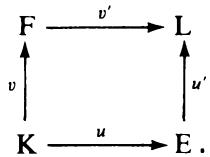
\includegraphics[keepaspectratio]{images/part001_e6455da9.jpg}}

By replacing \((L, u')\) by an isomorphic extension of E we may suppose that L contains E as subfield and that \(u'\) is the canonical injection of E in L. By changing notation we thus obtain the following scholium:

SCHOLIUM. --- Let K and E be two fields and u a homomorphism of K into E. If K' is a field containing K as subfield, there exists a field E' containing E as subfield and a homomorphism u' of K' into E' extending u.
